%!TEX root = ../dissertation.tex

\section*{Общая характеристика работы} %\addcontentsline{toc}{section}{Общая характеристика работы}

%!TEX root = ../dissertation.tex
\textbf{Актуальность темы.} 

\textbf{Степень разработанности темы.}

\textbf{Целью} исследования является разработка точных методов генерации детерминированных конечных автоматов по имеющимся примерам поведения с использованием сокращения пространства поиска при решении задачи выполнимости.

Для~достижения указанной цели определены следующие \textbf{задачи}:
\begin{enumerate}
  \item Разработать точный метод построения ДКА по имеющимся примерам поведения с использованием <<компактных>> предикатов нарушения симметрии на основе алгоритма обхода графа в ширину.
  \item Разработать методы сокращения пространства поиска при решении задачи выполнимости для 
  построения ДКА по имеющимся примерам поведения, основанные на структурных особенностях искомого автомата.
  \item Разработать точный метод построения всех возможных ДКА по имеющимся примерам поведения с использованием программных средств решения задачи выполнимости.
  \item Разработать комбинированный точный метод построения ДКА по имеющимся примерам поведения на основе сведения к задаче выполнимости и с использованием подхода уточнения абстракции по контрпримерам.
  \item Разработать программный комплекс, реализующий все вышеуказанные методы.
  \item Провести экспериментальные исследования для оценки применимости и времени работы разработанных и реализованных методов, изложенных выше. 
\end{enumerate}

\textbf{Объект исследования}~{---} методы генерации конечных автоматных моделей.

\textbf{Предмет исследования}~{---} точные методы генерации детерминированных конечных автоматов по имеющимся примерам поведения.

\textbf{Соответствие паспорту специальности.} Данная диссертация соответствует пункту 5 <<\textbf{Разработка и исследование моделей и алгоритмов анализа данных, обнаружения закономерностей в данных и их извлечениях разработка и исследование методов и алгоритмов анализа текста}, устной речи и изображений.>>.

\emph{??? пункт 10 <<\textbf{Разработка основ} математической теории языков и грамматик, \textbf{теории конечных автоматов} и теории графов.>>}

\emph{??? пункт 7 <<\textbf{Разработка методов} распознавания образов, фильтрации, \textbf{распознавания и синтеза} изображений, \textbf{решающих правил}. Моделирование формирования эмпирического знания.>>}

\emph{??? пункт 3 <<Исследование методов и разработка средств кодирования информации в виде данных. Принципы создания языков описания данных, языков манипулирования данными, языков запросов. \textbf{Разработка и исследование моделей данных и новых принципов их проектирования}>>.}

\textbf{Основные положения, выносимые на~защиту:}
\begin{enumerate}
  \item Разработан точный метод построения ДКА по имеющимся примерам поведения с использованием <<компактных>> предикатов нарушения симметрии на основе алгоритма обхода графа в ширину.
  \item Разработаны методы сокращения пространства поиска при решении задачи выполнимости для построения ДКА по имеющимся примерам поведения, основанные на структурных особенностях искомого автомата.
  \item Разработан точный метод построения всех возможных ДКА по имеющимся примерам поведения с использованием программных средств решения задачи выполнимости.
  \item Разработан комбинированный точный метод построения ДКА по имеющимся примерам поведения на основе сведения к задаче выполнимости и с использованием подхода уточнения абстракции по контрпримерам.
\end{enumerate}

\textbf{Научная новизна} заключается в~следующем:
\begin{enumerate}
  \item Впервые точный метод построения ДКА по имеющимся примерам поведения с использованием предикатов нарушения симметрии на основе алгоритма обхода графа в ширину был предложен научным руководителем В.И.~Ульянцевым при участии автора диссертации.
  Новизна предложенного в данной работе метода заключается в использовании <<компактных>> предикатов нарушения симметрии --- пропозициональное кодирование данных предикатов на языке задачи выполнимости содержит квадратичное относительно размера автомата количество дизъюнктов вместо кубического из оригинального метода.
  Разработанный метод помимо уменьшения размера булевой формулы обеспечивает статистически значимое преимущество скорости работы по сравнению с существующими точными методами.
  \item Впервые были предложены методы сокращения пространства поиска при решении задачи выполнимости для построения ДКА по имеющимся примерам поведения, основанные на структурных особенностях искомого автомата.
  Использование данных методов обеспечивает статистически значимое преимущество скорости работы по сравнению с существующими точными методами. 
  \item Впервые был предложен точный метод построения всех возможных ДКА по имеющимся примерам поведения с использованием программных средств решения задачи выполнимости.
  Новизна предложенного метода заключается в использовании предикатов нарушения симметрии на основе алгоритма обхода графа в ширину, что позволяет оставить для рассмотрения единственного представителя для каждого класса эквивалентности по изоморфизму.
  \item Впервые был предложен комбинированный точный метод построения ДКА по имеющимся примерам поведения на основе сведения к задаче выполнимости и с использованием подхода уточнения абстракции по контрпримерам.
  Новизна предложенного метода заключается в использовании только части имеющихся примеров поведения при построении ДКА, что обеспечивает статистически значимое преимущество скорости работы по сравнению с существующими точными методами в случаях, когда число имеющихся примеров поведения излишне велико относительно размера искомого автомата.
\end{enumerate}

\textbf{Методология и методы исследования.} В работе используются методы теории автоматов, теории сложности, дискретной математики, объектно-ориентированное программирование, методы проведения и анализа экспериментальных исследований

\textbf{Достоверность} полученных результатов, подтверждается корректным обоснованием постановок задач, точной формулировкой критериев, а также результатами проведенных экспериментальных исследований по использованию предложенных в диссертации методов.

\textbf{Теоретическая значимость работы} состоит в том, что для задачи генерации ДКА по имеющимся примерам поведения было предложено пропозициональное кодирование предикатов нарушения симметрии на основе алгоритма обхода графа в ширину, содержащее асимптотически меньшее количество дизъюнктов.
Также для задачи генерации ДКА по имеющимся примерам поведения были предложены методы по сокращению пространства поиска при решении задачи выполнимости.
Помимо этого, был предложен метод для решения задачи построения всех различных неизоморфных ДКА по имеющимся примерам поведения, для решения которой ранее эффективных методов не существовало.
Также был предложен метод, объединяющий в себе два различных подхода: сведение к задаче выполнимости и уточнение абстракции по контрпримерам.

\textbf{Практическая значимость работы} состоит в том, что разработанные методы и реализованные в рамках программного комплекса на основе данных методов алгоритмы  позволяют ускорить и улучшить генерацию ДКА по имеющимся примерам поведения, что позволяет решать задачи более высокой сложности, выраженной в размере искомого автомата, в размере алфавита, в недостаточном или избыточном покрытии автомата примерами поведения.

\textbf{Участие в научно-исследовательских работах.} 
Результаты диссертации использовались при проведении НИР <<Разработка эффективных методов машинного обучения для построения детерминированных конечных автоматов на основе решения задачи выполнимости>> (грант РФФИ <<Мой первый грант>> 18-37-00425, 2018--2020 гг.) под руководством автора диссертации.

Полученные результаты также использовались при проведении следующих НИР:
\begin{itemize}
  \item <<Биоинформатика, машинное обучение, технологии программирования, теория кодирования, проактивные системы>> (субсидия \mbox{074-U01} в рамках государственной финансовой поддержки ведущих университетов Российской Федерации, 2013--2017 гг.);
  \item <<Методы, модели и технологии искусственного интеллекта в биоинформатике, социальных медиа, киберфизических, биометрических и речевых системах>>, (субсидия \mbox{08-08} в рамках государственной финансовой поддержки ведущих университетов Российской Федерации, 2018--2020 гг.).
\end{itemize}

\textbf{Апробация результатов работы.}
Основные результаты работы докладывались на следующих конференциях и семинарах:
\begin{enumerate}
  \item 9\textsuperscript{th} International Conference on Language and Automata Theory and Applications (LATA 2015). 2015, Ницца, Франция.
  \item 6\textsuperscript{th} International Symposium ``From Data to Models and Back (DataMod)''. 2017, Тренто, Италия.
  \item 13\textsuperscript{th} International Conference on Language and Automata Theory and Applications (LATA 2019). 2015, Санкт-Петербург.
  \item IV-VII Всероссийский Конгресс молодых ученых. 2015-2018, Санкт-Петербург.
  \item IX Конгресс молодых ученых. 2020, Санкт-Петербург.
  \item XLVI Научная и учебно-методическая Конференция Университета \mbox{ИТМО}. 2017, Санкт-Петербург.
  \item XLVIII Научная и учебно-методическая Конференция Университета ИТМО. 2019, Санкт-Петербург.
\end{enumerate}

\textbf{Личный вклад автора.}.
  Идея точного метода построения ДКА по имеющимся примерам поведения с использованием <<компактных>> предикатов нарушения симметрии на основе алгоритма обхода графа в ширину принадлежит совместно автору диссертации и Ж.~Маркешу-Сильве, реализация алгоритма на базе предложенного метода принадлежит лично автору диссертации, проведение вычислительных экспериментов принадлежит совместно автору диссертации и А.И.~Игнатьеву.
  Идея методов сокращения пространства поиска при решении задачи выполнимости для построения ДКА по имеющимся примерам поведения, основанные на структурных особенностях искомого автомата принадлежит совместно автору диссертации и Ж.~Маркешу-Сильве, реализация алгоритмов на базе предложенных методов принадлежит лично автору диссертации, проведение вычислительных экспериментов принадлежит совместно автору диссертации и А.И.~Игнатьеву.
  Идея точного метода построения всех возможных ДКА по имеющимся примерам поведения с использованием программных средств решения задачи выполнимости принадлежит совместно автору диссертации и научному руководителю В.И.~Ульянцеву, реализация алгоритма на базе предложенного метода и проведение вычислительных экспериментов принадлежит лично автору.
  Идея комбинированного точного метода построения ДКА по имеющимся примерам поведения на основе сведения к задаче выполнимости и с использованием подхода уточнения абстракции по контрпримерам принадлежит совместно автору диссертации и научному руководителю В.И.~Ульянцеву, реализация алгоритма на базе предложенного метода и проведение вычислительных экспериментов принадлежит лично автору.

\textbf{Публикации.}
Основные результаты по теме диссертации изложены в девяти публикациях, из них три опубликованы в изданиях, индексируемых в базе цитирования Scopus, одна публикация издана в журнале, рекомендованном ВАК.
Также у автора диссертации имеются две публикации по другим темам, из которых одна связана с машинным обучением, другая с построением автоматных моделей для кибер-физических систем, обе опубликованы в изданиях, индексируемых в базе цитирования Scopus.

\newpage

\section*{Содержание работы}

Во \textbf{введении} диссертационной работы обоснована актуальность проводимых исследований. Сформулированы цель, задачи и положения, выносимые на защиту. Изложена научная новизна и практическая значимость результатов, полученных в диссертационной работе.

%------

\textbf{\underline{Первая глава}} диссертации посвящена обзору предметной области и результатов существующих исследований, посвященных генерации детерминированных конечных автоматов.
Кроме того, в первой главе приведены терминология, основные определения и известные результаты ряда разделов информатики, необходимых для описания предлагаемых в диссертации методов и алгоритмов.

\insection{\ref{sec:review:sat}} приведена формальная постановка задачи выполнимости булевой формулы, даны необходимые определения, и представлено краткое описание основных подходов к ее решению.
Также в данном разделе описан подход к решению NP-трудных задач с помощью полиномиального сведения таких задач к задаче выполнимости.
Помимо этого, приводится краткий обзор существующих программных средств решения SAT.

Булева формула задана в \emph{конъюнктивно-нормальной форме} (КНФ), если является конъюнкцией дизъюнктов~--- множества литералов, связанных дизъюнкцией.
\emph{Задача выполнимости булевой формулы} (\emph{задача выполнимости}, \emph{boolean satisfiability problem}~{---} SAT) заключается в определении, существует ли выполняющая подстановка для некоторой булевой формулы заданной в КНФ.
Задача выполнимости является исторически первой, для которой была доказана NP-трудность~--- любую задачу из класса NP можно за полиномиальное время свести к SAT.
Данный факт объясняет актуальность разработки все более эффективных программных средств для решения задачи выполнимости.
Ежегодно в научном сообществе проходят соревнования по выяснению лучшего программного средства для решения SAT, что также способствует постоянному развитию данной области.
В основе современных программных средств лежит стратегия \emph{управляемого конфликтами обучения дизъюнктов} (\emph{conflict-driven clause learning}, CDCL).

Подход к решению задачи из класса NP, когда разрабатывается сведение к SAT и затем используется современное программное средство для поиска выполняющей подстановки, зачастую оказывается заметно эффективнее и проще, чем разработка применимого на практике метода, решающего непосредственно исходную задачу.
Еще одним немаловажным достоинством такого подхода является тот факт, что достаточно единожды написать сведение к SAT, а затем без прикладывания каких-либо усилий пользоваться развитием программных средств, выбирая самое эффективное из них.

\insection{\ref{sec:review:cegar}} приведено описание алгоритма уточнения абстракции по контрпримерам (counterexample guided abstraction refinement~{---} CEGAR). 
Методы, использующие данный алгоритм применимы в ситуации, когда необходимо построить модель, соответствующую заданным требованиям, имея при этом доступ к некоторой проверяющей системе~--- оракулу. 
На начальном шаге строится некоторая, возможно, случайная модель.
Затем начинается итеративный процесс уточнения имеющейся модели~--- на каждом шаге текущая модель проверяется оракулом на соответствие заданным требованиям. 
Если проверка проходит успешно, то модель найдена.
Иначе, оракул сообщает один или несколько контрпримеров, которые затем используются для уточнения модели.

\insection{\ref{sec:review:dfa-inf}} приведены даны базовые понятия о детерминированных конечных автоматах и постановка задачи генерации детерминированных конечных автоматов по примерам поведения. 
Примерами поведения некоторого ДКА $\mathcal{D}$ называются два множества слов, состоящих из символов алфавита автомата, $S_{+}$ и $S_{-}$ таких, что все слова из $S_{+}$ принадлежат языку $\mathcal{L}\left(\mathcal{D}\right)$, то есть должны им приниматься, а все слова из $S_{-}$ не принадлежат языку $\mathcal{L}\left(\mathcal{D}\right)$, то есть должны им отвергаться.
Задача генерации ДКА по примерам поведения заключается в поиске автомата минимального размера (с минимальным числом состояний), соответствующего имеющимся примерам поведения.
Ранее было доказано, что настоящая задача является NP-полной, ровно как и задача генерации ДКА любого фиксированного размера, соответствующего имеющимся примерам поведения.
Пример детерминированного конечного автомата, соответствующего наборам примеров поведения $S_{+} = \{aba, bb, bba\}$ и $S_{-} = \{b, ba\}$, представлен на рисунке~\ref{syn:img:dfa-ex}.
Можно заметить, что автомата размера два, соответствующего множествам $S_{+}$ и $S_{-}$, не существует.

\begin{figure}[ht]
  \centering
  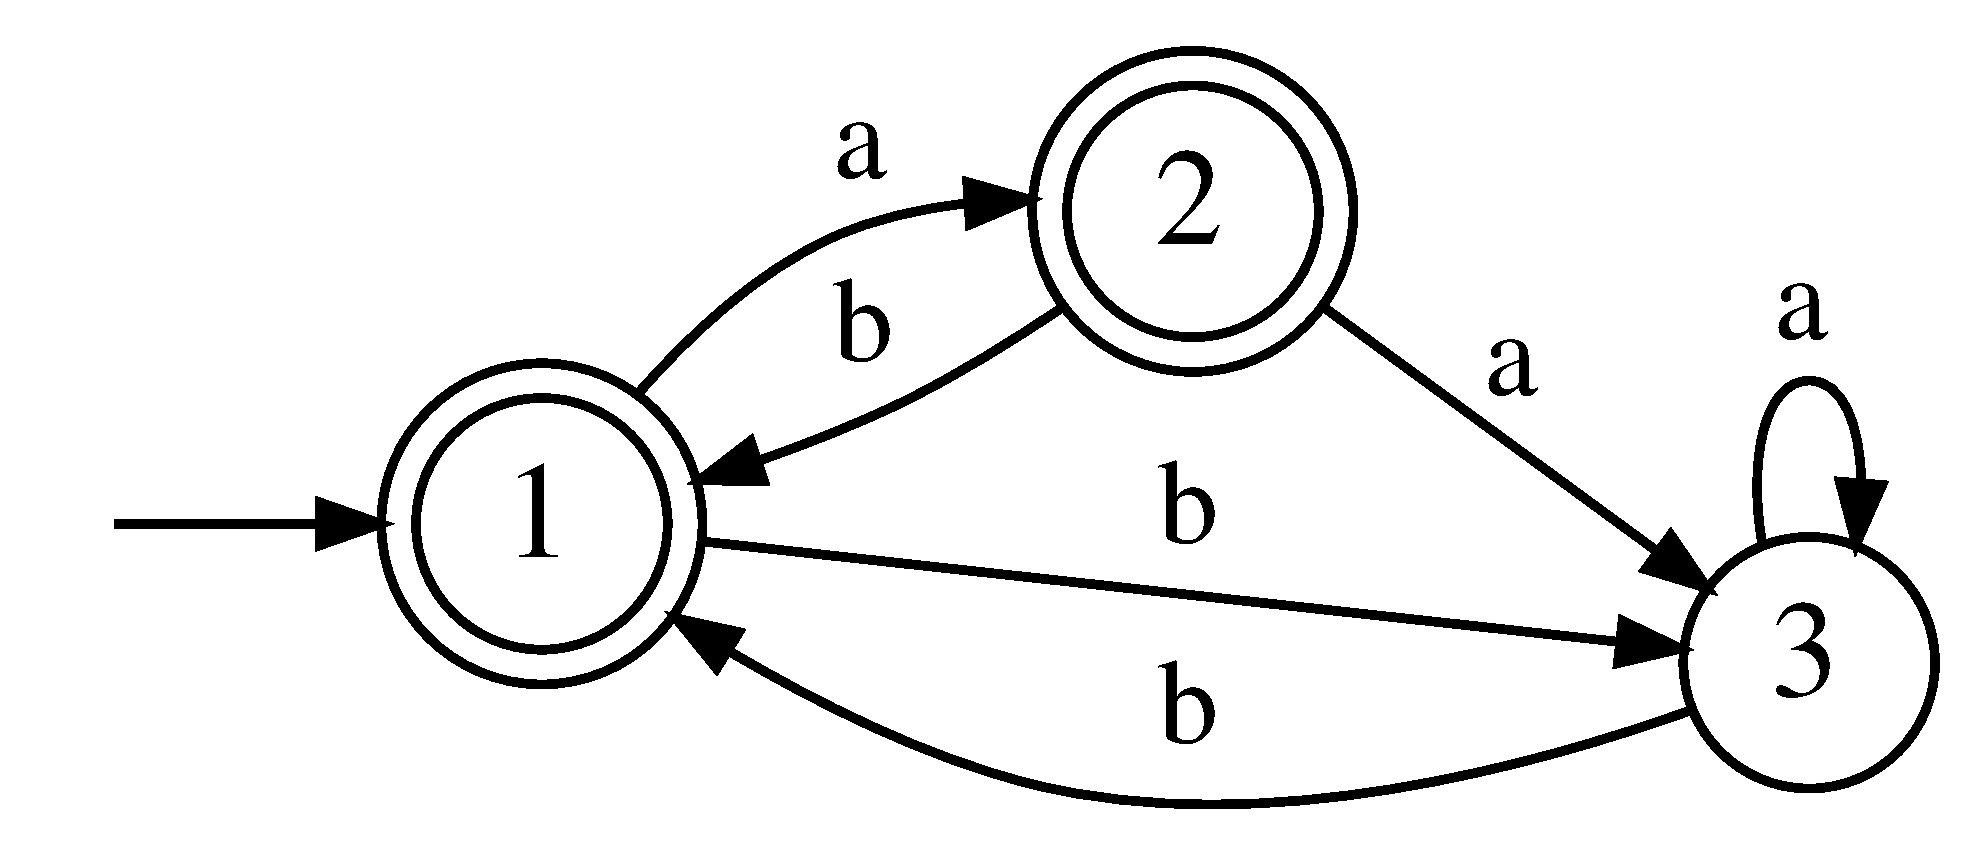
\includegraphics[scale=0.16]{img/datamod/FIG1.eps}
  \caption{Пример ДКА минимального размера, соответствующего наборам примеров поведения $S_{+} = \{aba, bb, bba\}$ и $S_{-} = \{b, ba\}$}
  \label{syn:img:dfa-ex}
\end{figure}


\insection{\ref{sec:review:heuristic-dfa-inf}} приведен обзор существующих эвристических и метаэвристических методов генерации детерминированных конечных автоматов по примерам поведения. 

Среди эвристических алгоритмов можно выделить алгоритм \emph{объединения состояний на основе свидетельств} (\emph{evidence-driven state merging}~--- EDSM).
Среди метаэвристических алгоритмов можно выделить эволюционные стратегии, генетические алгоритмы и муравьиные алгоритмы.

Следует отметить, что данные походы являются неточными~--- ими не гарантируется, что найденный автомат содержит минимальное возможное число состояний, а иногда вообще не гарантируется, что какой-то автомат будет найден.


\insection{\ref{sec:review:sat-dfa-inf}} приведен обзор существующих методов генерации детерминированных конечных автоматов по примерам поведения, основанных на сведении к SAT. В отличие от эвристических и метаэвристических подходов, данные методы являются точным~--- гарантируется, что автомат, соответствующий примерам поведения, будет построен за конечное время и будет содержать минимальное возможное число состояний.

Первым шагом рассматриваемых методов является построение расширенного префиксного дерева (augmented prefix tree acceptor~--- APTA)~--- древовидной структуры данных, основанной на обычном префиксном дереве, в которой каждая вершина либо не помечена, либо помечена как допускающая или отвергающая. 
Пример расширенного префиксного дерева представлен на рисунку~\ref{syn:img:apta-ex}.

\begin{figure}[ht]
  \centering
  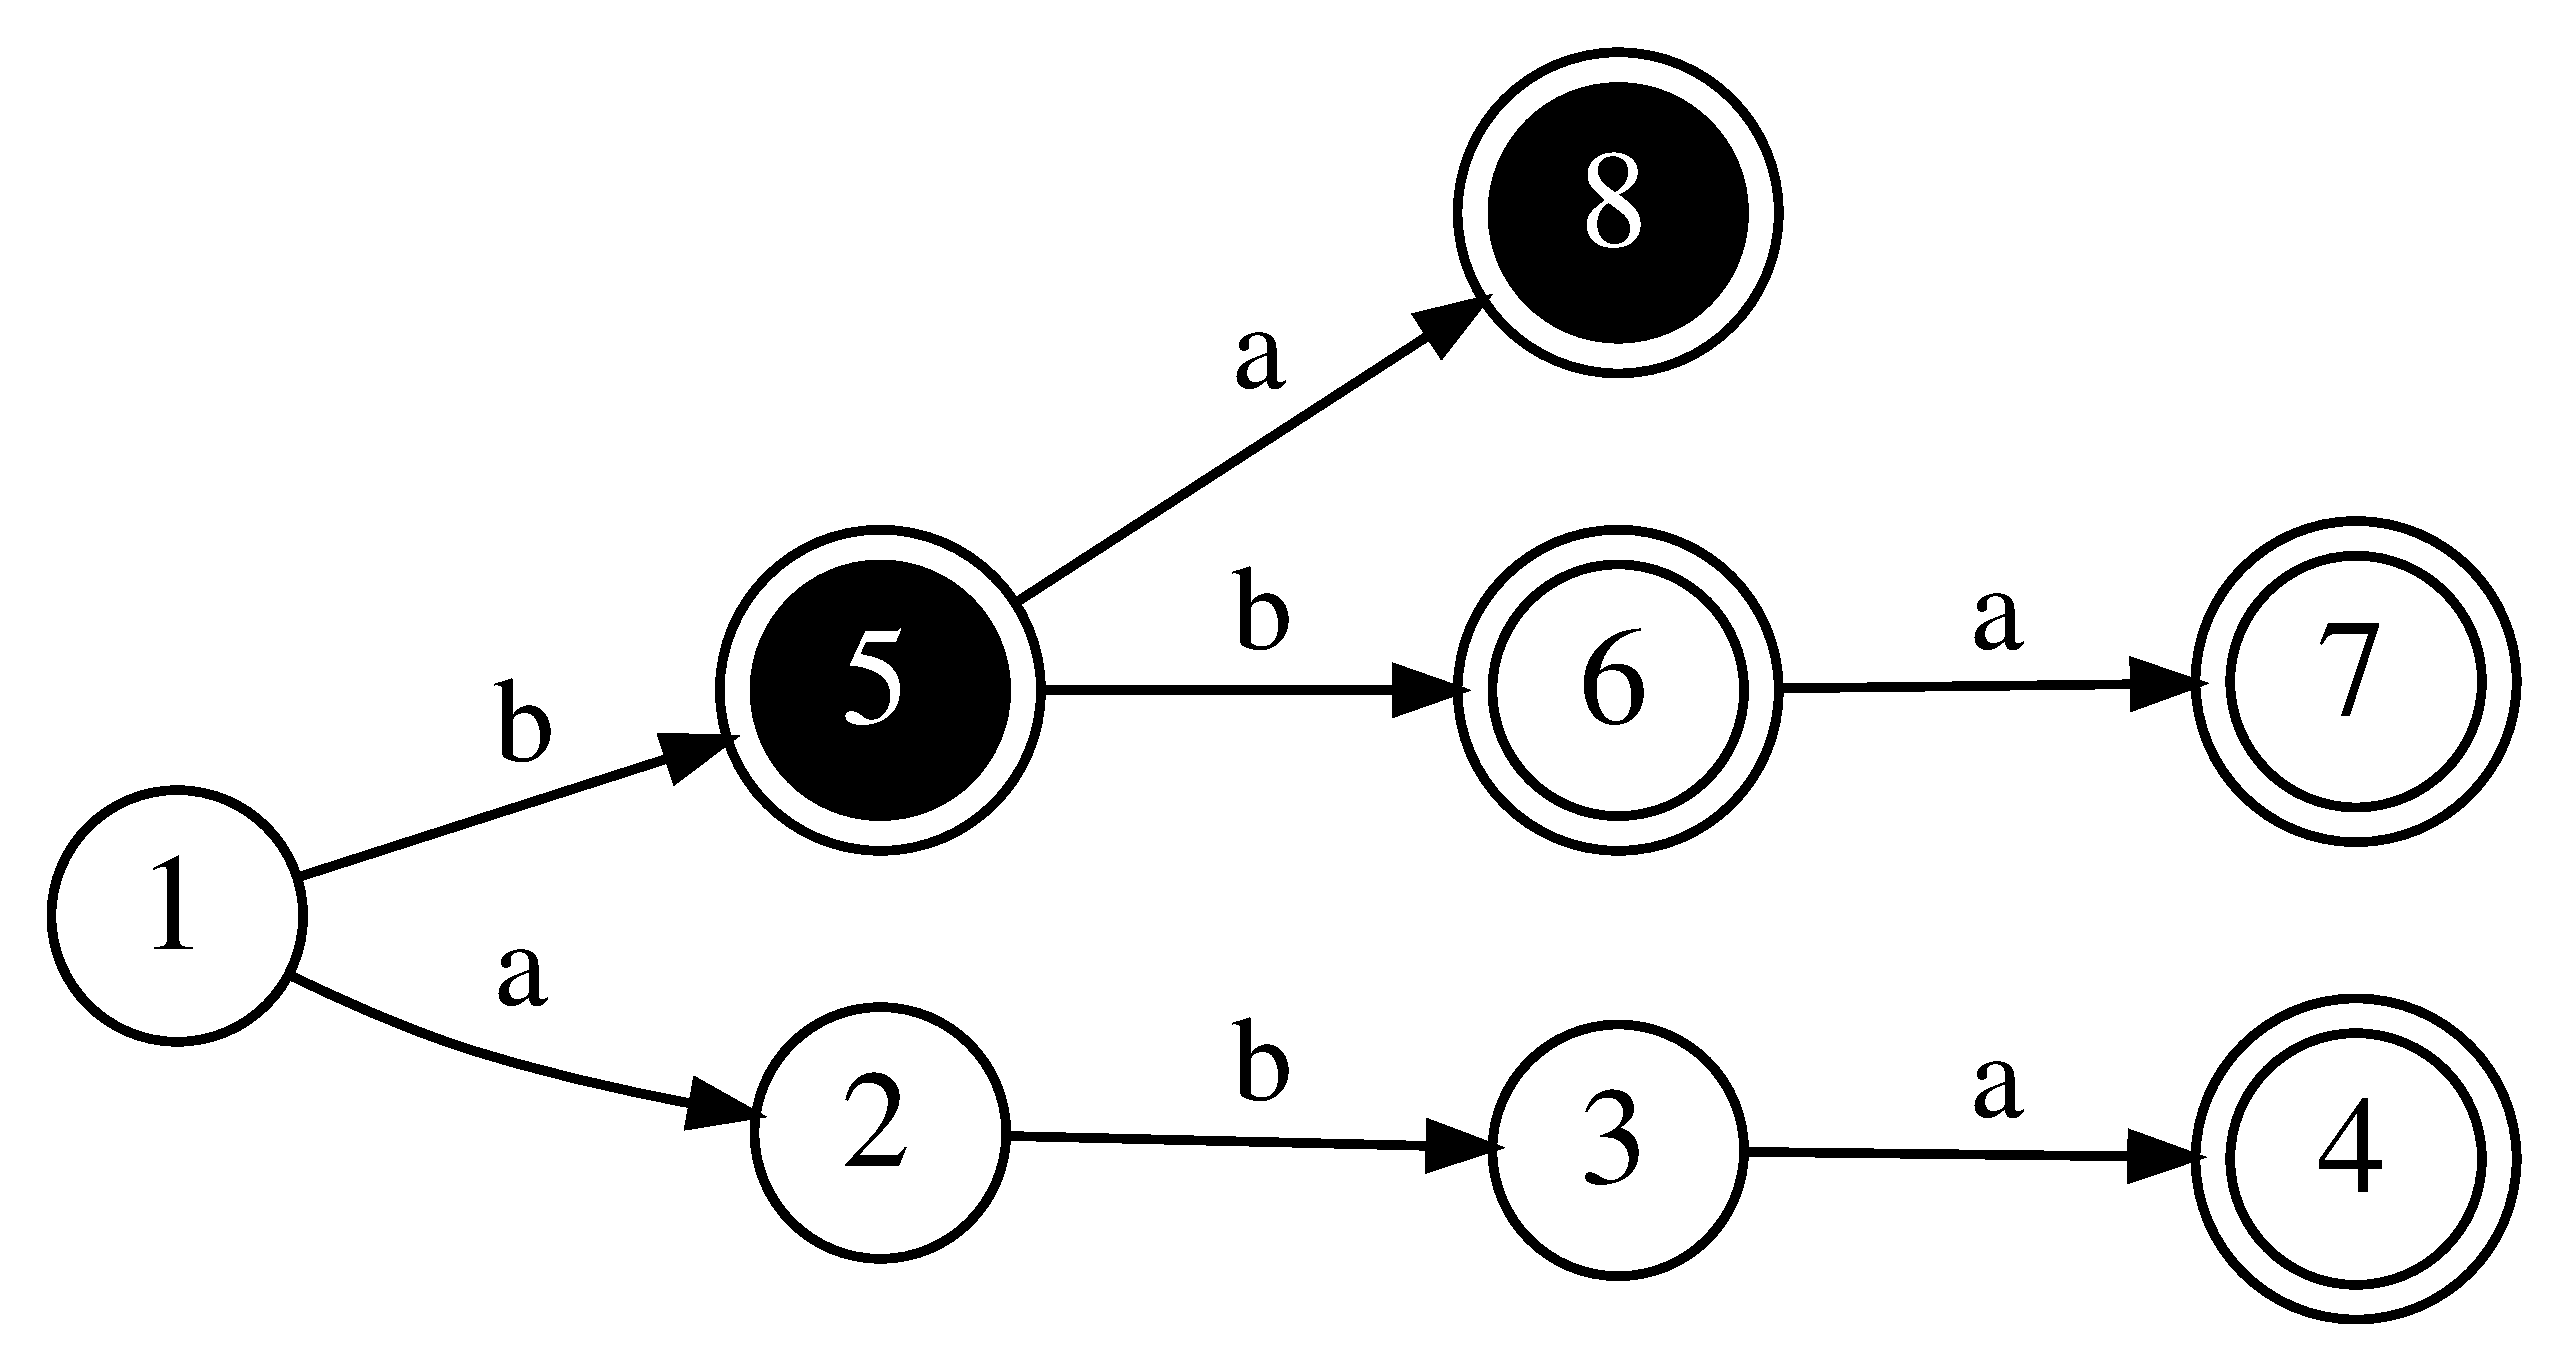
\includegraphics[scale=0.14]{img/datamod/FIG2a.eps}
  \caption{Пример расширенного префиксного дерева, построенного по наборам примеров поведения $S_{+} = \{aba, bb, bba\}$ и $S_{-} = \{b, ba\}$}
  \label{syn:img:apta-ex}
\end{figure}

Далее, начиная с некоторой нижней оценки на размер~--- в простейшем случае с единицы~--- происходит поиск автомата текущего размера, соответствующего построенному расширенному префиксному дереву. 
Данный процесс продолжается до тех пор, пока не будет найден ДКА, удовлетворяющий заданным требованием.
Итеративный перебор размера от меньшего к большему гарантирует, что найденный автомат имеет минимальный размер.
Как уже было сказано, задача поиска ДКА конкретного размера по заданным словарям принадлежит классу NP, а значит, может быть решена путем сведения к некоторой NP-трудной задаче.
Самым производительным точным методом до недавнего времени являлся \texttt{DFASAT}~\cite{heule-icgi10}, в котором авторы предложили сначала свести задачу генерации ДКА к задаче раскраски графа~--- необходимо раскрасить расширенное префиксное дерево в минимальное количество цветов так, чтобы все вершины одного цвета объединялись в одно состояние,~--- которую затем свести к задаче выполнимости.
Схема метода \texttt{DFASAT} представлена на рисунке~\ref{syn:img:dfasat-algo}.

\begin{figure}[ht]
  \centering
  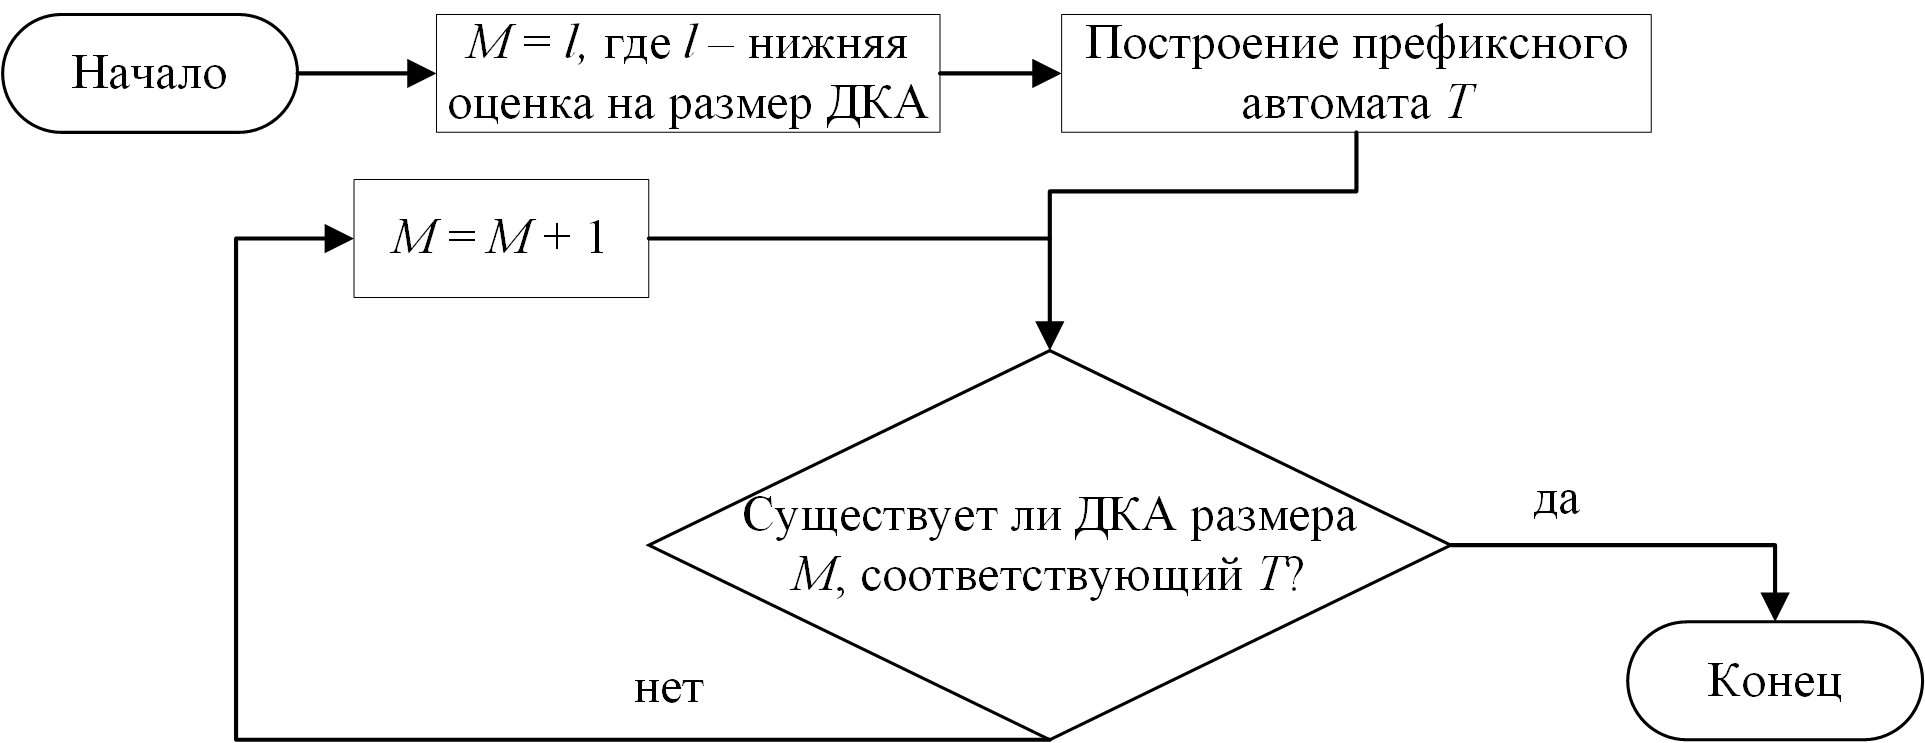
\includegraphics[scale=0.5]{img/ntv/basic.jpg}
  \caption{Схема точного метода генерации ДКА по заданным примерам поведения на основе сведения к SAT~--- \texttt{DFASAT}}
  \label{syn:img:dfasat-algo}
\end{figure}

Развитием данного метода занималась группа научного руководителя диссертанта В.~И.~Ульянцев, предложив использование предикатов нарушения симметрии на основе алгоритма обхода графа в ширину~\cite{zakirzyanov2015LATA}.
Дальнейшему улучшению метода посвящена настоящая диссертация.

\insection{\ref{sec:review:sym-breaking}} приведен обзор существующих подходов к сокращению пространства поиска при решении задачи выполнимости для генерации детерминированных конечных автоматов по примерам поведения.
Авторы \texttt{DFASAT} используют несколько различных подходов к сокращению пространства поиска. 
Во-первых, добавление нескольких видов дополнительных дизъюнктов в булеву формулу, которые не влияют на решение, но добавляют дополнительные ограничения на возможные значения переменных.
Во-вторых, построение графа совместимости, позволяющего заранее найти некоторые пары вершин префиксного дерева, которые не могут быть объединены в одно состояние автомата.
В-третьих, нахождение некоторой большой клики в графе совместимости и фиксирование нумерации вершин данной клики.

Использование вышеперечисленных подходов позволяет значительно увеличить производительность оригинального метода, однако они не решают фундаментальной проблемы наличия изоморфных автоматов.
Два автомата называются изоморфными, если они различаются только нумерацией состояний.
Таким образом, если ДКА содержит $N$ состояний, то существует $\mathcal{O}\left(N\right)$ изоморфных ему автоматов.
Несмотря на то, что изоморфные автоматы не отличаются с практической точки зрения, с точки зрения программного средства для решения SAT, они различны.

Решением данной проблемы стала разработка предикатов нарушения симметрии на основе \emph{обхода графа в ширину} (\emph{breadth-first search}~--- BFS)~\cite{zakirzyanov2015LATA}.
Добавление таких предикатов в булеву формулу фиксирует нумерацию рассматриваемых автоматов в порядке BFS, что для каждого класса эквивалентности по изоморфизму позволяет оставить для рассмотрения единственного представителя.
Для записи предикатов в виде булевой формулы требуется $\mathcal{O}\left(M^{3} + M^{2} \times L^{2}\right)$ дизъюнктов, где $N$~--- размер префиксного дерева, $M$~--- размер искомого ДКА.
Метод генерации ДКА при помощи сведения к SAT с использованием BFS предикатов нарушения симметрии является самым производительным точным методом, который лежит в основе всех методов, разрабатываемых в данной диссертации.
Пример BFS пронумерованного ДКА представлен на рисунке~\ref{syn:img:bfs:bfs-ex}, а на рисунке~\ref{syn:img:bfs:bfs-tree} представлено его дерево обхода.

\begin{figure}[ht]
  \centering
  \subfloat[Пример BFS пронумерованного автомата\label{syn:img:bfs:bfs-ex}]{
    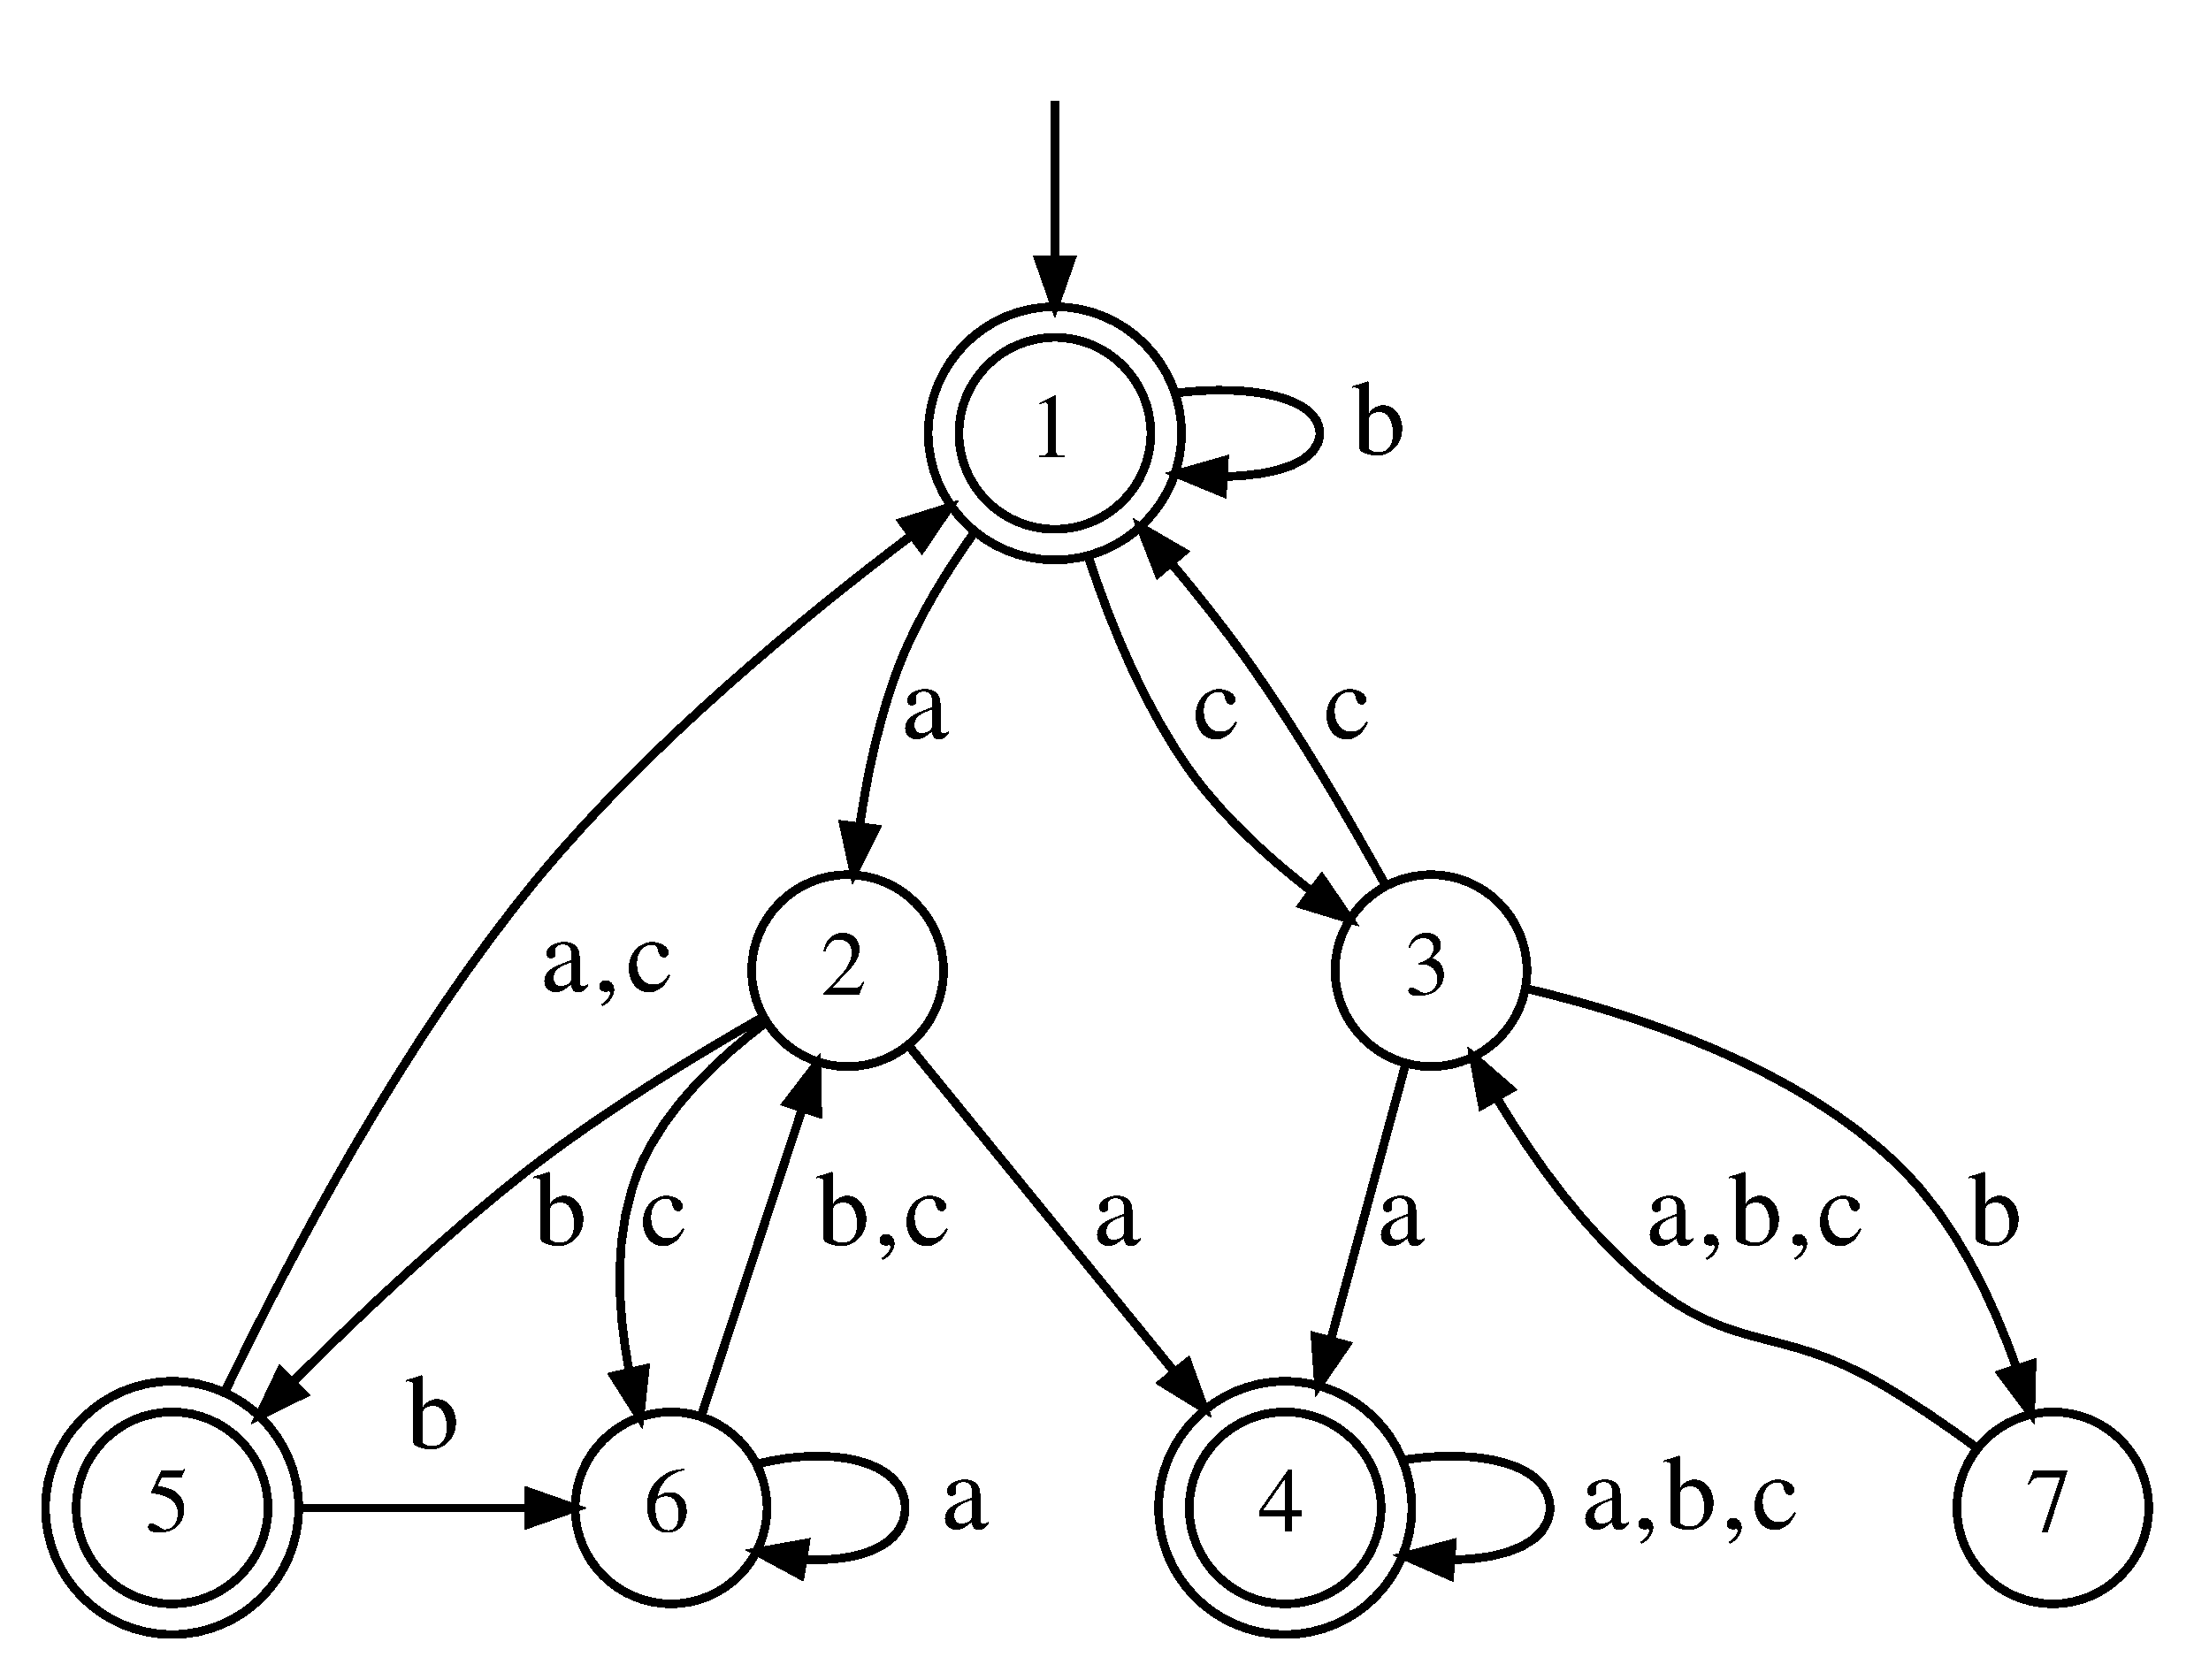
\includegraphics[scale=0.15]{img/datamod/BFS-example.eps}
  }
  \hfill
  \subfloat[Дерево BFS для автомата, представленного на рисунке~\ref{syn:img:bfs:bfs-ex}\label{syn:img:bfs:bfs-tree}]{
    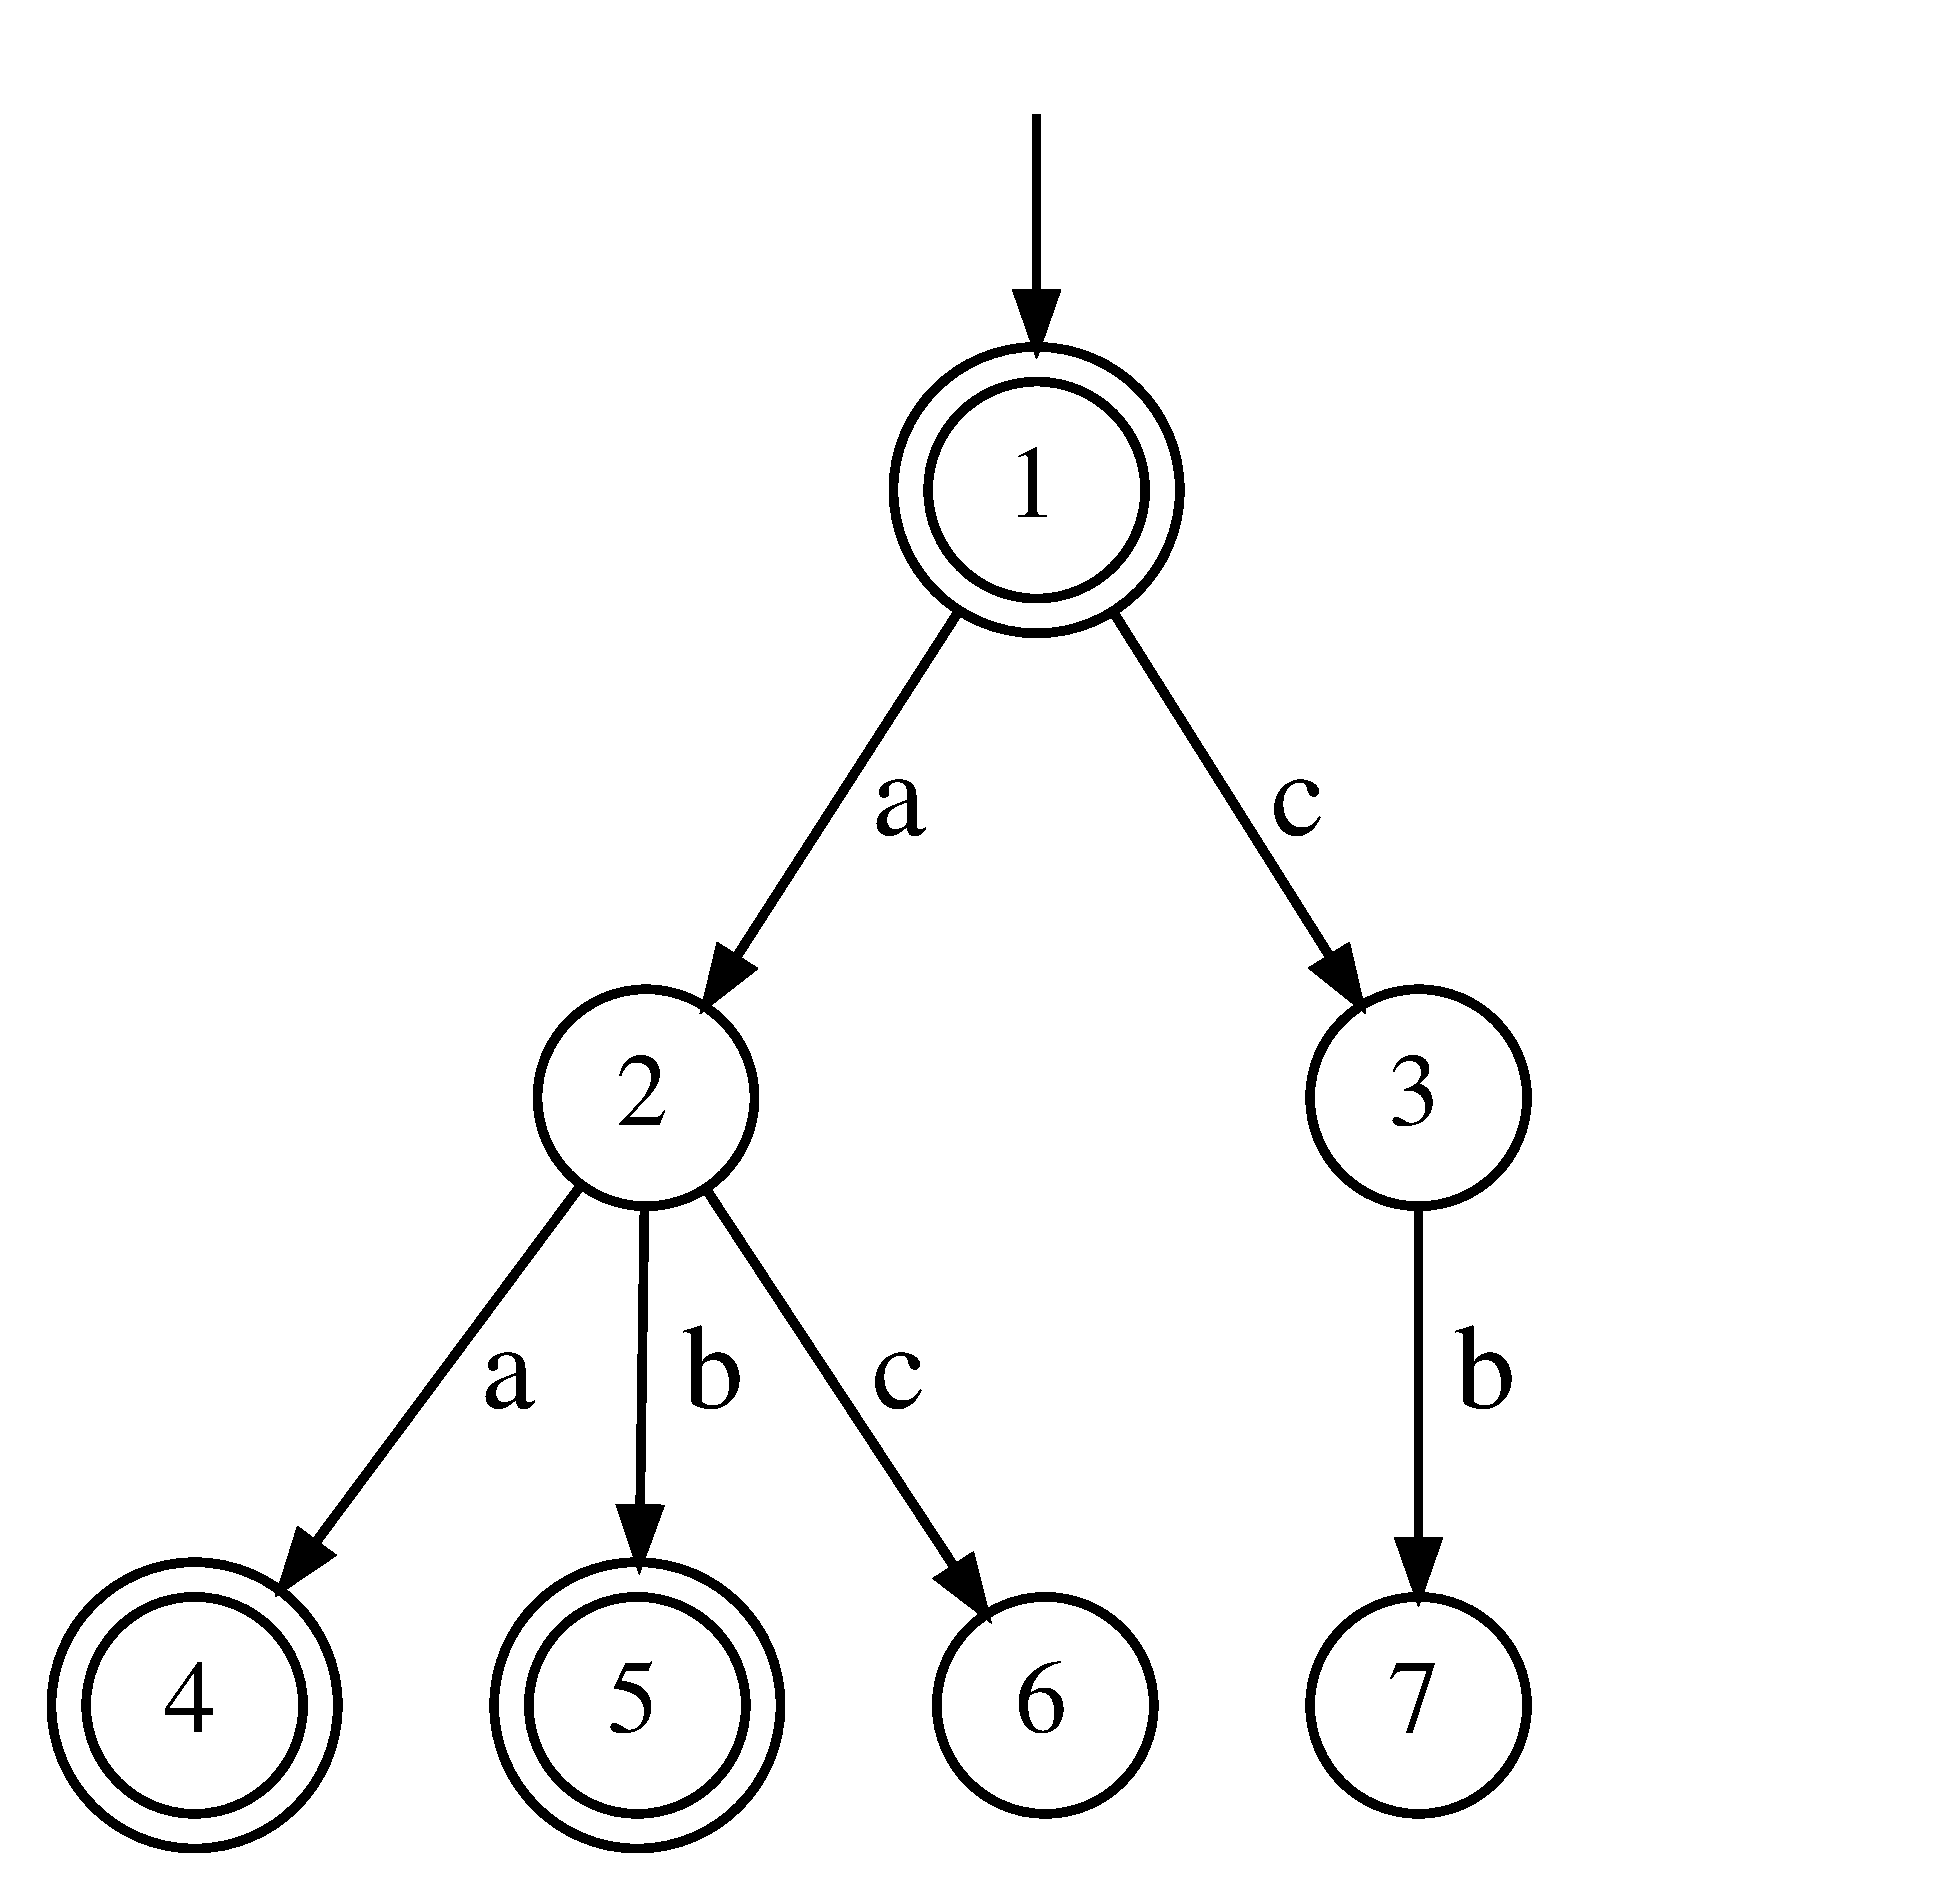
\includegraphics[scale=0.15]{img/datamod/BFS-tree.eps}
  }
  \caption{Пример BFS пронумерованного автомата и соответствующего BFS дерева}
  \label{syn:img:bfs}
\end{figure}

\insection{\ref{sec:review:tasks}} на основе результатов обзора формулируются задачи, решаемые в настоящей диссертационной работе.

%------

Во \textbf{\underline{второй главе}} настоящей диссертации описываются разработка, реализация и экспериментальные исследования методов генерации детерминированных конечных автоматов с использованием различных подходов к сокращению пространства поиска при решении задачи выполнимости.

\insection{\ref{sec:space:dfs}} приведено описание разработанных предикатов нарушения симметрии на основе алгоритма обхода графа в глубину (\emph{depth-first search}~--- DFS). 
Использование предикатов нарушения симметрии, задающих BFS нумерацию автомата, позволило значительно улучшить производительность метода \texttt{DFASAT}.
Логичной следующей задачей научного исследования было разработать предикаты нарушения симметрии на основе алгоритма DFS и метод, использующий их.
\inote{сюда добавить немного мяса}
Пример DFS пронумерованного ДКА представлен на рисунке~\ref{syn:img:dfs:dfs-ex}, а на рисунке~\ref{syn:img:dfs:dfs-tree} представлено его дерево обхода.

\begin{figure}[ht]
  \centering
  \subfloat[Пример DFS пронумерованного автомата\label{syn:img:dfs:dfs-ex}]{
    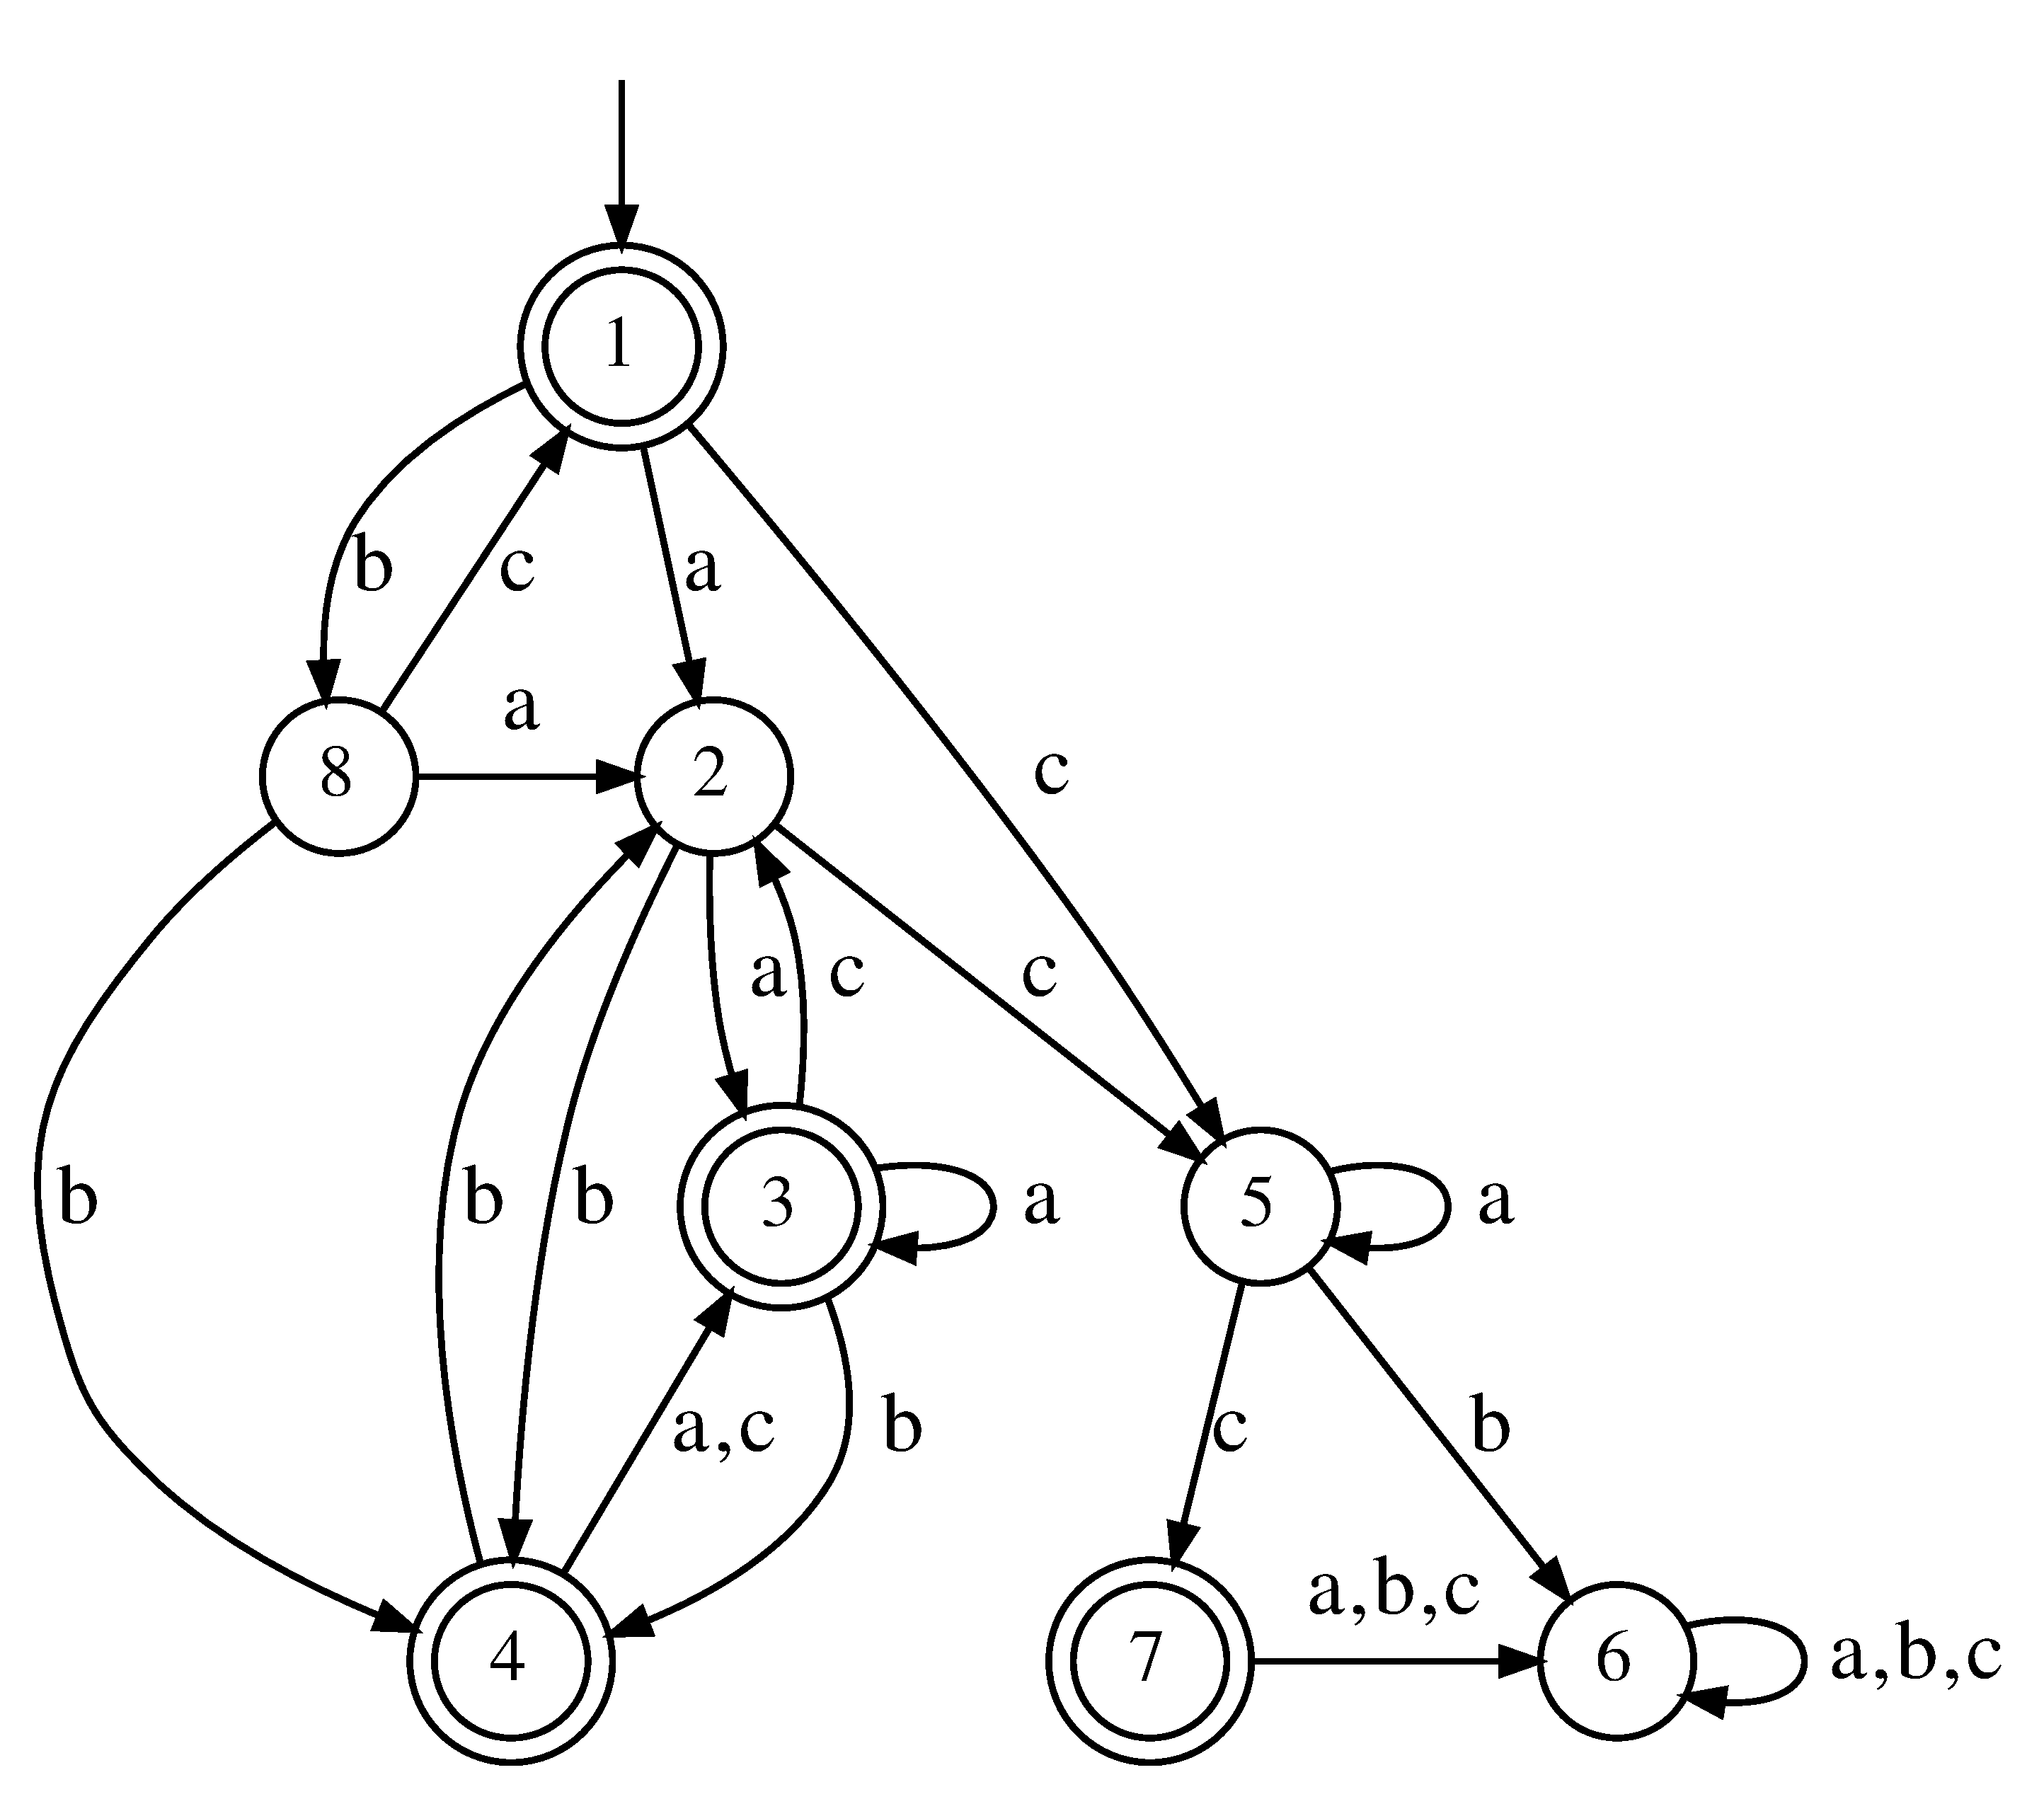
\includegraphics[scale=0.15]{img/datamod/DFS-example.eps}
  }
  \hfill
  \subfloat[Дерево DFS для автомата, представленного на рисунке~\ref{syn:img:dfs:dfs-ex}\label{syn:img:dfs:dfs-tree}]{
    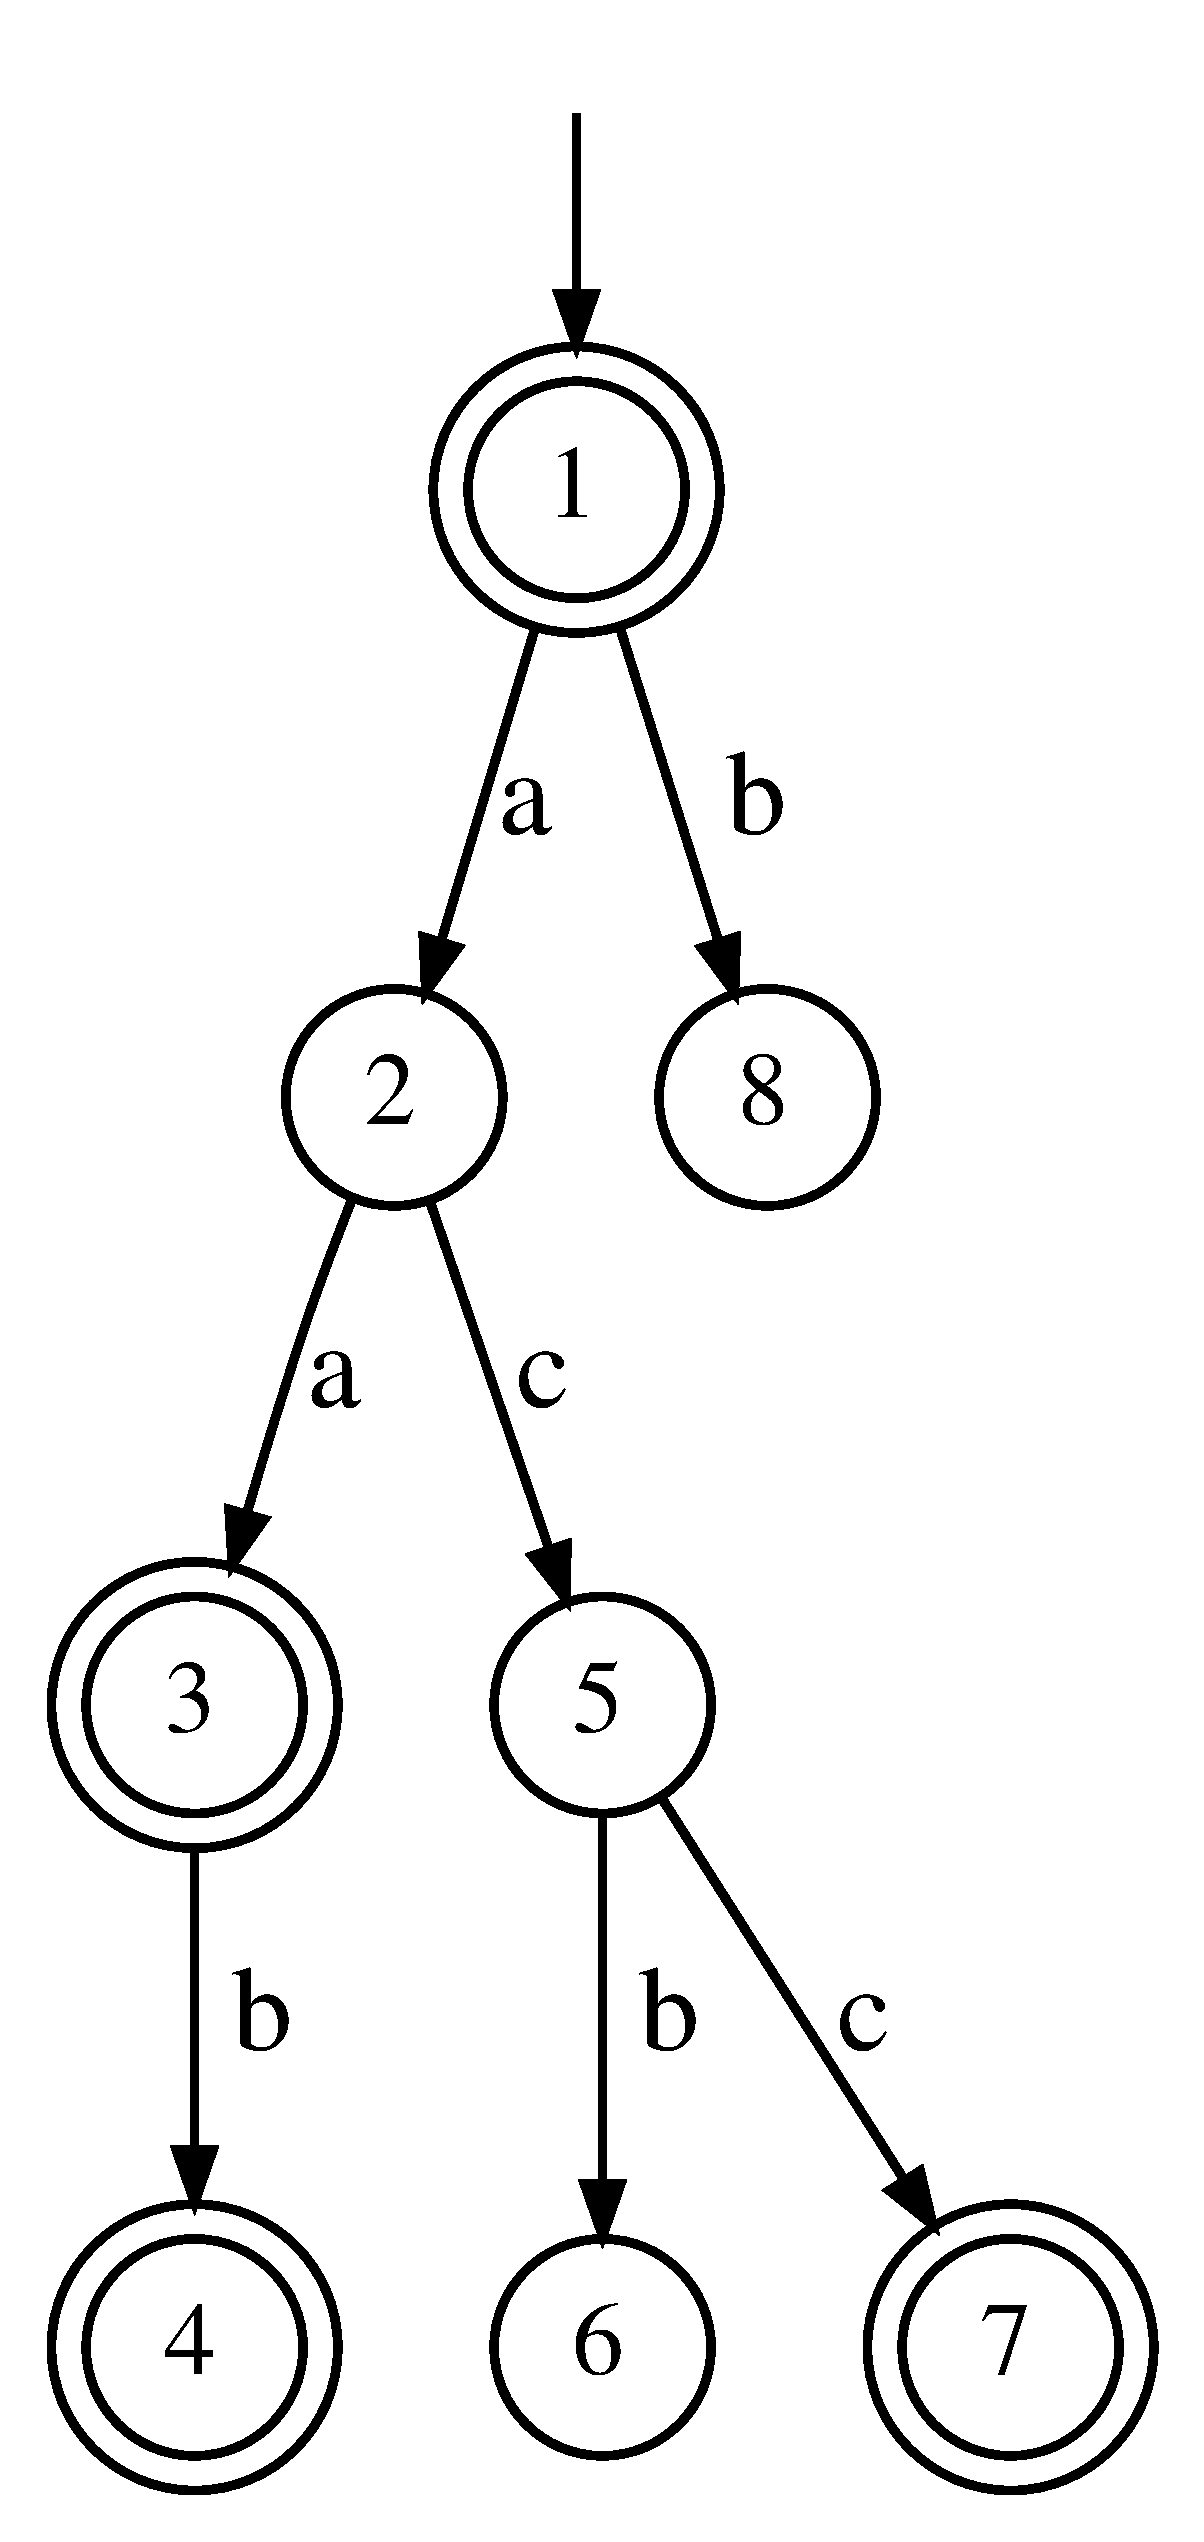
\includegraphics[scale=0.15]{img/datamod/DFS-tree.eps}
  }
  \caption{Пример DFS пронумерованного автомата и соответствующего BFS дерева}
  \label{syn:img:dfs}
\end{figure}

Разработанные предикаты выражаются КНФ-формулой, содержащей $\mathcal{O}\left(M^{4} + M^{3} \times L^{2}\right)$ факториалов, что на степень $M$ больше чем предикаты, задающие BFS нумерацию ДКА.

\insection{\ref{sec:space:tight}} приведено описание разработанных компактных предикатов нарушения симметрии на основе алгоритма BFS.
\inote{Возможно стоит везде поменять на ``разработаны методы''} 

Компактность разработанных предикатов заключается в том, что удалось сократить размер формулы, выражающей предикаты нарушения симметрии, задающие BFS нумерацию автомата, с $\mathcal{O}\left(M^{3} + M^{2} \times L^{2}\right)$ дизъюнктов до $\mathcal{O}\left(M^{2} \times L\right)$ дизъюнктов.
Анализ ограничений исходного сведения, которые выражались через $\mathcal{O}\left(M\right)$ и $\mathcal{O}\left(M^{2} \times L^{2}\right)$ дизъюнктов, показал, что часть параметров, задающих размер формулы являются независимыми, в то время как другие параметры могут быть исключены с помощью добавления новых переменных. 
Для каждого такого ограничения был разработан способ сделать его более компактным, что и позволило сократить общий размер формулы.
Помимо этого, б\emph{о}льшая часть дизъюнктов из оригинального сведения, которые состояли из $\mathcal{O}\left(M\right)$ литералов
были заменены на дизъюнкты, состоящие из двух или трех литералов, что заметно влияет на производительность программного средства для решения SAT, так как такие дизъюнкты обрабатываются за константное время и не хранятся в памяти~\cite{MSilva-SATbook09}.

\insection{\ref{sec:space:pruning}} приведено описание разработанных подходов к сокращению пространства поиска при генерации детерминированных конечных автоматов, основанных на особенностях структуры BFS дерева, а также на связях между расширенным префиксным деревом и искомом ДКА.
На рисунке~\ref{syn:img:full-bfs} представлено полное BFS дерево произвольного размера над произвольным алфавитом размера $L$.
Дерево названо полным, так как каждая вершина имеет ровно $L$ детей.

\begin{figure}[ht]
  \centering
  \scalebox{0.625}{%
\begin{tikzpicture}[scale=0.75, level 1/.style={sibling distance=60mm},level 2/.style={sibling distance=40mm}, level distance=25mm, level 3/.style={sibling distance=50mm}]
\node [ellipse,draw] (root){$1$}
  child {node [ellipse,draw] (a0) {$2$}
    child {node [ellipse,draw] (a0b0) {$L+2$}}
    child {node [ellipse,draw] (a0bj) {$L+j+1$}}
    child {node [ellipse,draw] (a0bL) {$2L+1$}}
  }
  child {node (aj) {$\vdots$}
    child {node [ellipse,draw] (r) {$r$}
      child {node [xshift=-0.25em,ellipse,draw] (r0) {$(r-1)L+2$}}
      child {node [ellipse,draw] (rj) {$(r-1)L+j+1$}}
      child {node [xshift=0.25em,ellipse,draw] (rL) {$rL+1$}}
    }
  }
  child {node [ellipse,draw] (aL) {$L+1$}
    child {node [ellipse,draw] (aLb0) {$L^2+2$}}
    child {node [ellipse,draw] (aLbj) {$L^2+j+1$}}
    child {node [ellipse,draw] (aLbL) {$L^2+L+1$}}
  }
;

\path (root) -- (a0) node [below, midway, darkblue] {$1$};
\path (root) -- (aL) node [below, midway, darkblue] {$L$};

\path (a0) -- (a0b0) node [below, midway, darkblue] {$1$};
\path (a0) -- (a0bj) node [left, midway, darkblue] {$j$};
\path (a0) -- (a0bL) node [below, midway, darkblue] {$L$};

\path (aL) -- (aLb0) node [below, midway, darkblue] {$1$};
\path (aL) -- (aLbj) node [left, midway, darkblue] {$j$};
\path (aL) -- (aLbL) node [below, midway, darkblue] {$L$};

\path (r) -- (r0) node [below, midway, darkblue] {$1$};
\path (r) -- (rj) node [left, midway, darkblue] {$j$};
\path (r) -- (rL) node [below, midway, darkblue] {$L$};

\path (a0) -- (aj) node [midway] {$..$};
\path (aj) -- (aL) node [midway] {$..$};

\path (a0b0) -- (a0bj) node [midway] {$..$};
\path (a0bj) -- (a0bL) node [midway] {$..$};

\path (aLb0) -- (aLbj) node [midway] {$..$};
\path (aLbj) -- (aLbL) node [midway] {$..$};

\path (r0) -- (rj) node [midway] {$..$};
\path (rj) -- (rL) node [midway] {$..$};
\end{tikzpicture}
%
%
\begin{comment}
%
%
\begin{figure}
\centering
\begin{tikzpicture}[scale=0.75, level 1/.style={sibling distance=60mm},level 2/.style={sibling distance=40mm}, level distance=25mm, level 3/.style={sibling distance=50mm}]
\node [ellipse,draw] (root){$1$}
  child {node [ellipse,draw] (a0) {$2$}
   child {node [ellipse,draw] (a0b0) {$L+2$}}
   child {node [ellipse,draw] (a0bj) {$L+j+2$}}
   child {node [ellipse,draw] (a0bL) {$2L+1$}}
  }
  child {node (aj) {$\vdots$}
    child {node [ellipse,draw] (r) {$r$}
      child {node [ellipse,draw] (r0) {$(r-1)L+2$}}
      child {node [ellipse,draw] (rj) {$(r-1)L+j+2$}}
      child {node [ellipse,draw] (rL) {$rL+1$}
        child [grow=right,red] {node [red] (j) {$0\leq j < L$} edge from parent[draw=none]}
      }
    }
  }
  child {node [ellipse,draw] (aL) {$L+1$}
    child {node [ellipse,draw] (aLb0) {$L^2+2$}}
    child {node [ellipse,draw] (aLbj) {$L^2+j+2$}}
    child {node [ellipse,draw] (aLbL) {$L^2+L+1$}}
  }
;

\path (root) -- (a0) node [midway, red] {$0$};
\path (root) -- (aL) node [midway, red] {$L-1$};

\path (a0) -- (a0b0) node [midway, red] {$0$};
\path (a0) -- (a0bj) node [midway, red] {$j$};
\path (a0) -- (a0bL) node [midway, red] {$L-1$};

\path (aL) -- (aLb0) node [midway, red] {$0$};
\path (aL) -- (aLbj) node [midway, red] {$j$};
\path (aL) -- (aLbL) node [midway, red] {$L-1$};

\path (r) -- (r0) node [midway, red] {$0$};
\path (r) -- (rj) node [midway, red] {$j$};
\path (r) -- (rL) node [midway, red] {$L-1$};

\path (a0) -- (aj) node [midway] {$..$};
\path (aj) -- (aL) node [midway] {$..$};

\path (a0b0) -- (a0bj) node [midway] {$..$};
\path (a0bj) -- (a0bL) node [midway] {$..$};

\path (aLb0) -- (aLbj) node [midway] {$..$};
\path (aLbj) -- (aLbL) node [midway] {$..$};

\path (r0) -- (rj) node [midway] {$..$};
\path (rj) -- (rL) node [midway] {$..$};
\end{tikzpicture}
\caption{Worst case BFS tree with $0\leq j <L$}
\end{figure}
%
%
\end{comment}
}
  \caption{Полное BFS дерево, где $\abs{\Sigma}=L$}
  \label{syn:img:full-bfs}
\end{figure}

После анализа данного дерева были сформулированы некоторые свойства и ограничения свойственные BFS-дереву.
Например, было доказано, что у некоторой вершины с номером $r$ в полном дереве самый правый ребенок имеет номер $rL + 1$.
Далее было доказано, что тогда $rL + 1$ является верхней оценкой на номер ребенка вершины $r$ в произвольном BFS дереве.
Тогда, можно утверждать, что в произвольном BFS дереве у вершины с номером $r$ дети могут иметь номера только в диапазоне от $r + 1$ до $rL + 1$.
Введение данных ограничений позволяет сократить число используемых в сведении переменных и сократить размер получающейся формулы.

Помимо этого, можно заметить, что в любом BFS дереве дети любой вершины $r$ имеют последовательные номера, а также их, что очевидно, не более чем $L$.
Было разработано кодирование данного свойства на языке SAT.
Кодирование данного свойства на языке SAT и добавление его в формулу позволяет дополнительно сократить пространство поиска при решении задачи выполнимости.

\inote{рисунок и описание связи между APTA и DFA}

\insection{\ref{sec:space:results}} приведены описание разработанного  на языке \emph{python} программного средства \texttt{DFA-Inductor-py}, предназначенного для генерации детерминированных конечных автоматов, описание реализации разработанных методов как частей данного программного средства, а также результаты экспериментальных исследований всех разработанных методов. 

\inote{Кратко про средство}

Были проведены две серии экспериментальных исследований.
Сначала сравнивались метод генерации ДКА по заданным примерам поведения с использованием оригинальных предикатов нарушения симметрии на основе BFS и аналогичный метод с использованием DFS предикатов.
Дополнительно в сравнение был включен метод \texttt{DFASAT}, использующий в качестве предикатов нарушения симметрии фиксирование нумерации некоторой большой клики графа несовместимости, так как он лежит в основе двух других методов. 
Результаты экспериментов представлены в таблице~\ref{syn:tab:DFS-results} и позволяют сделать вывод, что использование DFS предикатов нарушения симметрии нецелесообразно, так как метод, их использующий, значительно проигрывает методу, использующему BFS предикаты.
Однако можно заметить, что метод, использующий DFS предикаты значительно выигрывает в производительности относительно метода \texttt{DFASAT}.
Тем не менее, исходя из результатов, было решено не продолжать развитие DFS предикатов и сосредоточиться на улучшении предикатов, использующих алгоритм обхода графа в ширину.

\begin{table}[ht]
  \caption{Медианное время работы методов генерации ДКА по заданным примерам поведения с использованием BFS предикатов нарушения симметрии, DFS предикатов нарушения симметрии и метода \texttt{DFASAT} в секундах. Время работы методов было ограничено одним часом ($\text{TL} = 3600\,\, \text{секунд}$)}
  \centering
  \scalebox{0.95}{
    \begin{tabular}{cccccc}
      M & DFS     & & BFS    & & \texttt{DFASAT}\\
      \hline
      10 & 20.9   & & 20.5   & & 23.3  \\
      12 & 40.4   & & 37.6   & & 240.3 \\
      14 & 82.2   & & 62.4   & & TL    \\
      16 & 205.1  & & 114.1  & & TL    \\
      18 & 601.7  & & 181.9  & & TL    \\
      20 & 2501.6 & & 293.7  & & TL    \\
      22 & TL     & & 453.3  & & TL    \\
      24 & TL     & & 625.1  & & TL    \\
      26 & TL     & & 925.8  & & TL    \\
      28 & TL     & & 1314.4 & & TL    \\
      30 & TL     & & 1635.5 & & TL    \\
    \end{tabular}
  }
  \label{syn:tab:DFS-results}
\end{table}

Во втором экспериментальном исследовании сравнивались методы использующие оригинальные BFS предикаты (сейчас, называется \texttt{DFA-Inductor}, вероятно будет изменено позже) и BFS предикаты, разработанные в настоящей диссертации (сейчас, называется \texttt{DFA-Inductor~2}, точно будет изменено позже).
Как и ранее дополнительно в сравнение был включен метод \texttt{DFASAT}.
Результаты сравнения всех трех методов представлены на рисунке~\ref{syn:img:plots:cactus} и показывают, что метод \texttt{DFA-Inductor~2} способен за одно и то же время решить большее число экземпляров задачи генерации ДКА по заданным примерам поведения, чем метод \texttt{DFA-Inductor}.
Также можно видеть, что метод \texttt{DFASAT} не способен составить конкуренции двум другим подходам.

На рисунке~\ref{syn:img:plots:scatter} представлено детальное сравнение методов \texttt{DFA-Inductor} и \texttt{DFA-Inductor~2}, где видно, что при решении подавляющего числа экземпляров задачи генерации ДКА, второй метод показывает лучшие результаты.

\begin{figure}[ht]
  \centering
  \begin{subfigure}[b]{0.48\textwidth}
    \centering
    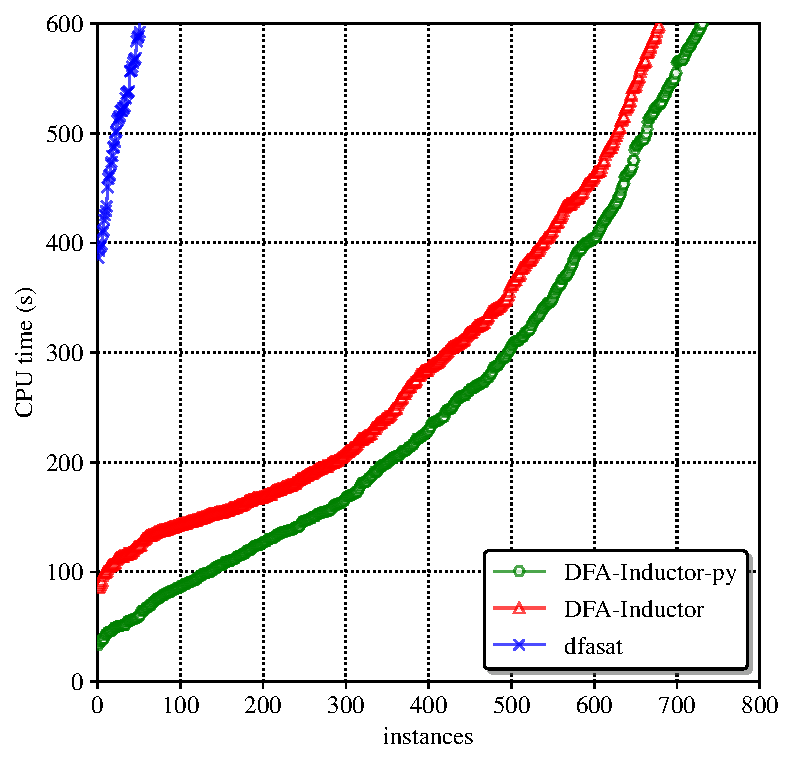
\includegraphics[width=\textwidth]{img/lata19/plots/cactus}
    \caption{Сравнение методов \texttt{DFA-Inductor}, \texttt{DFA-Inductor~2} и \texttt{DFASAT}, показывающее, число различных экземпляров задачи, решенное за определенное время}
    \label{syn:img:plots:cactus}
  \end{subfigure}%
  \;\;
  \begin{subfigure}[b]{0.48\textwidth}
    \centering
    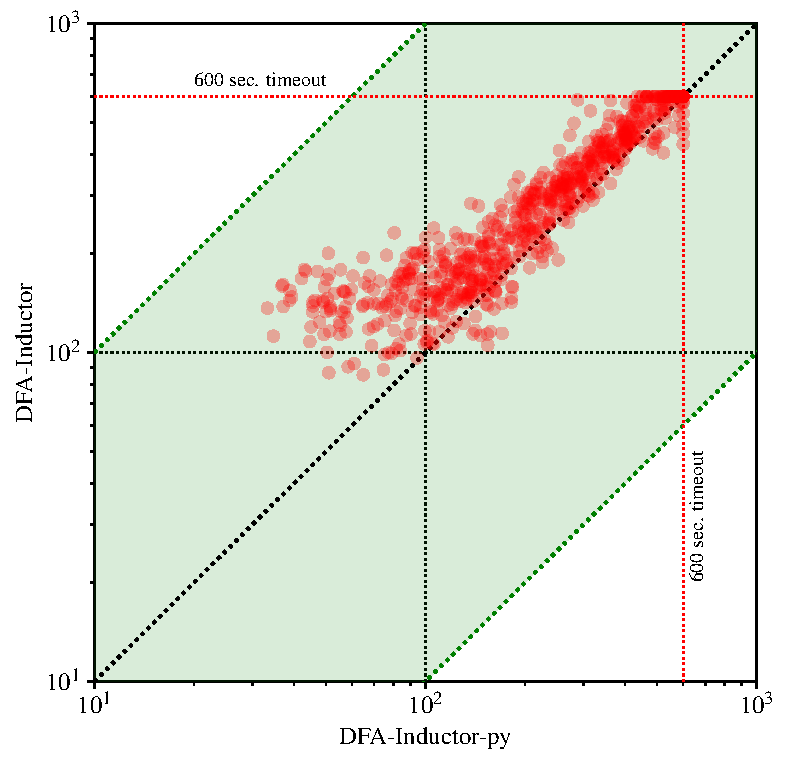
\includegraphics[width=\textwidth]{img/lata19/plots/scatter}
    \caption{Детальное сравнение методов \texttt{DFA-Inductor} и \texttt{DFA-Inductor~2}, сравнивающее их производительность в решении каждого экземпляра задачи}
    \label{syn:img:plots:scatter}
  \end{subfigure}
  \caption{Результаты сравнения метода, использующего оригинальные BFS предикаты (\texttt{DFA-Inductor}), метода, использующего новые BFS предикаты (\texttt{DFA-Inductor~2}), и \texttt{DFASAT}}
  \label{syn:img:plots}
\end{figure}

%------

В \textbf{\underline{третьей главе}} настоящей диссертации описываются разработка, реализация и экспериментальные исследования точного метода генерации детерминированных конечных автоматов по избыточному набору примеров поведения с использованием сведения к задаче выполнимости и подхода уточнения абстракции по контрпримерам.

\insection{\ref{sec:cegar:motivation}} приведено исследование границ применимости предложенных в предыдущих главах методов в зависимости от размера расширенного префиксного дерева. 
Размер булевой формулы, кодирующей задачу генерации ДКА, линейно зависит от размера префиксного дерева, конкретно~--- $\mathcal{O}\left(N \times M^{2}\right)$ дизъюнктов, где $N$~--- размер префиксного дерева, а $M$~--- размер генерируемого ДКА.
Число используемых переменных в булевой формуле также линейно зависит от размера префиксного дерева~--- $\mathcal{O}\left(N \times M + M^{2}\right) переменных.$
Таким образом, при неизменном генерируемом автомате, размер булевой формулы и число переменных может сильно меняться в зависимости от числа примеров поведения и их длины.
Программному средству для решения SAT при увеличении размера префиксного дерева становится все затратнее хранить формулу и работать с ней, а переменных для перебора становится все больше.
Это приводит к ситуации, когда один и тот же автомат может быть получен за секунды работы программного средства по небольшому числу примеров поведения небольшой длины и может быть не найден за часы и дни работы средства в случае \emph{избыточного} числа длинных примеров поведения.

Так как в случае детерминированных конечных автоматов ключевая информация о примере поведения~--- принимается данное слово автоматом или нет~--- содержится в последней вершине пути в расширенном префиксном дереве, соответствующего данному слову, то едва ли можно что-то сделать в случае длинных примеров поведения.
Однако, в случае избыточного числа примеров поведения, можно взять только часть из них и построить тот же автомат быстрее.
Сложность состоит в способе выбора примеров поведения, так как можно исключить те примеры, которые являются необходимыми для генерации того ДКА, который является ответом на исходную задачу, и получить совершенно другой автомат.
В следующем разделе предлагается метод итеративного выбора только значимых примеров поведения из всего изначального множества, решающий данную проблему.

\insection{\ref{sec:cegar:cegar-algo}} приведено описание разработанного точного метода генерации ДКА по избыточному набору примеров поведения на основе сведения к SAT и с использованием подхода CEGAR. 
Как было сказано в разделе~\ref{sec:review:cegar}, обычно алгоритм уточнения абстракции по контрпримерам применяется для решения задач активного обучения. 
Задача генерации ДКА по заданным примерам поведения в свою очередь относится к классу задач пассивного обучения.
Однако, в настоящей диссертации предлагается метод, решающий задачу генерации ДКА по заданным примерам, использующий идеи подхода CEGAR.

Как и классический алгоритм CEGAR, предлагаемый метод итеративно уточняет модель, которая в настоящей диссертации является детерминированным конечным автоматом.
Изначально расширенное префиксное дерево не содержит вершин, но будет достраиваться на каждом шаге.
На каждом шаге работы алгоритма предлагается с помощью сведения к SAT пытаться строить ДКА текущего размера по текущему префиксному дереву.
Если такой ДКА не существует, то как и раньше размер искомого автомата увеличивается на единицу и процесс поиска повторяется.
Если же такой автомат найден, он проверяется на соответствие всему множеству примеров поведения.
Если ДКА соответствует всем примерам поведения, то задача решена.
Иначе, среди тех примеров поведения, которым построенный автомат не соответствует, выбирается один или несколько контрпримеров, по которым достраивается префиксное дерево, строится новая булева формула и поиск продолжается.
Схема предложенного метода представлена на рисунке~\ref{syn:img:cegar-algo}.

\begin{figure}[ht]
  \centering
  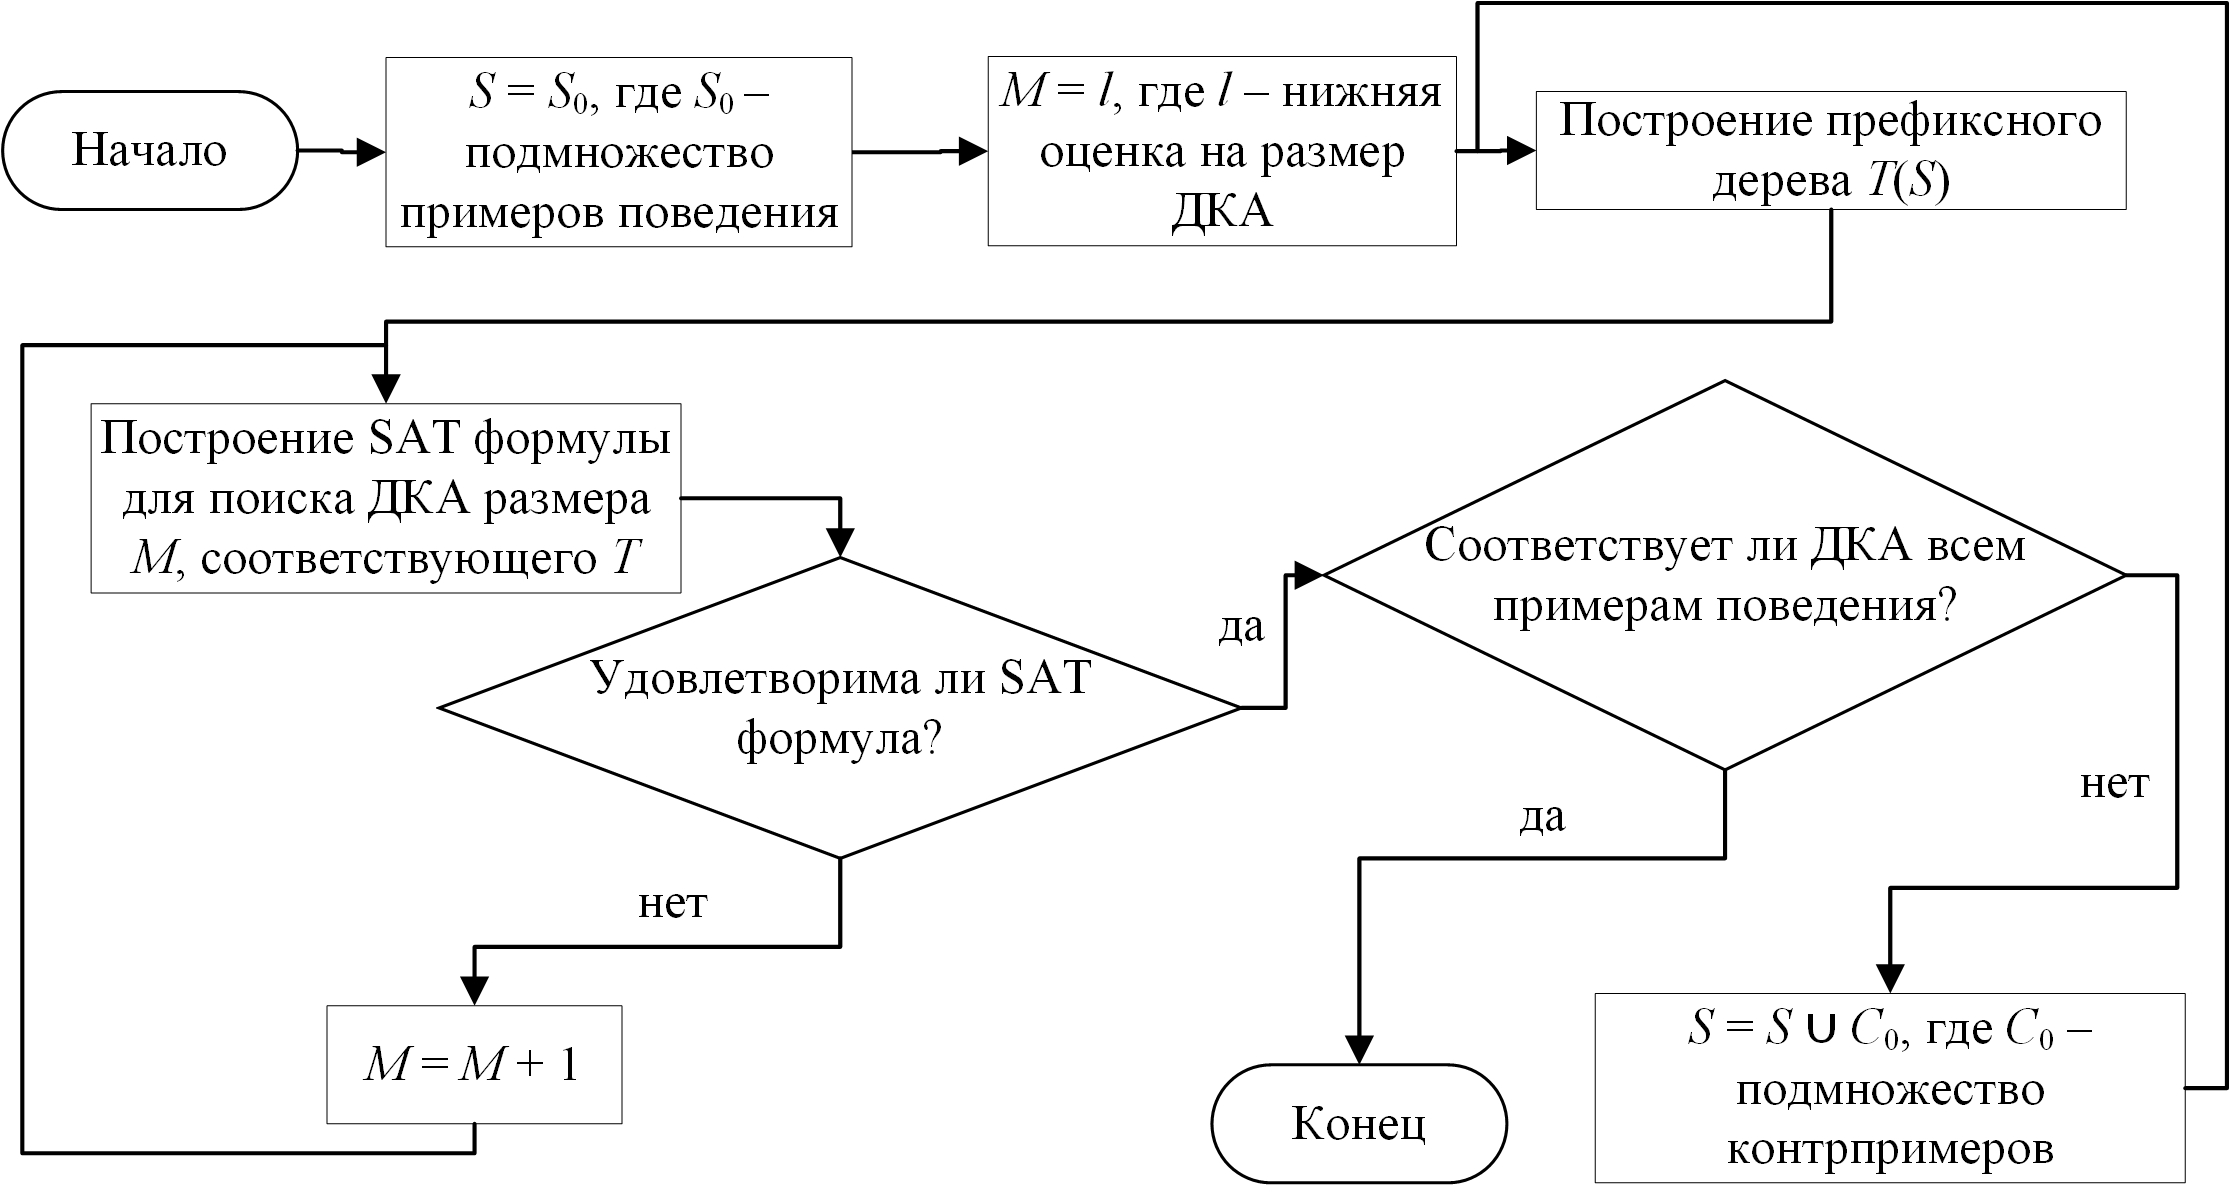
\includegraphics[scale=0.5]{img/ntv/cegar.jpg}
  \caption{Cхема точного метода генерации ДКА по избыточному набору примеров поведения на основе сведения к SAT и с использованием подхода CEGAR}
  \label{syn:img:cegar-algo}
\end{figure}

Необходимо заметить, что перезапускать программное средство для решения SAT при каждом достраивании префиксного дерева крайне неэффективно, так как при добавлении новых дизъюнктов в формулу, пространство поиска решения SAT только сужается, а значит нет необходимости начинать поиск выполняющей подстановки заново.
Можно использовать инкрементальные программные средства, которые после нахождения некоторой выполняющей подстановки переходят в режим ожидания новых дизъюнктов и затем продолжают поиск решения уже для новой уточненной формулы с того места, где остановились в прошлый раз.

\insection{\ref{sec:cegar:results}} приведены описание реализации разработанного метода как части программного средства \texttt{DFA-Inductor-py} и результаты экспериментальных исследований разработанного метода. 

\inote{добавить эксперименты}
\emph{Здесь будет график, показывающий, что при большом (и, вероятно, будет выявлено при каком именно) числе примеров поведения, подход, использующий CEGAR дает значительное преимущество.}

%------

В \textbf{\underline{четвертой главе}} настоящей диссертации дается постановка задачи генерации всех различных детерминированных конечных автоматов по заданным примерам поведения, а затем описываются разработка, реализация и экспериментальные исследования двух методов, решающих поставленную задачу. 

\insection{\ref{sec:findall:problem}} приведена формальная постановка задачи генерации всех неизоморфных ДКА минимального размера, удовлетворяющих заданным примерам поведения.
Как уже было показано ранее, ДКА минимального размера является максимально точным обобщением имеющихся данных, выраженных с помощью примеров поведения.
Однако в случае, когда примеры поведения недостаточно хорошо описывают искомый автомат, может существовать несколько различных удовлетворяющих автоматов минимального размера.
В таком случае рациональным решением может быть построить все такие автоматы для проведения дальнейшего анализа.
Важно отметить, что в данном случае слово ``различные'' употребляется как синоним слова ``неизоморфные''.

Ранее методов генерации всех различных ДКА минимального размера не предлагалось. 
Более того, без использования предикатов нарушения симметрии на основе BFS или DFS, разрешающих рассматривать для каждого класса эквивалентности по изоморфизму одного представителя вместо факториала, не представляется возможным генерация всех различных ДКА с помощью сведения к SAT.

\inote{возможно дать прямо постановку задачи формальную тут, раз это новая задача}

\insection{\ref{sec:findall:SAT-based}} приведено описание метода генерации всех неизоморфных ДКА минимального размера с использованием сведения к SAT и предикатов нарушения симметрии.
Так как при использовании предикатов нарушения симметрии на основе алгоритма BFS (ровно как и на основе алгоритма DFS) может быть сгенерирован только BFS пронумерованный ДКА, то достаточно заблокировать уже найденный автомат и исключить его (вместо со всеми изоморфными ему автоматами) из пространства поиска.
Из найденной выполняющей постановки построить автомат можно, используя только переменные переходов $y_{i,l,j}$ и переменные допуска $z_{i}$.
Тогда достаточно из всей найденной выполняющей подстановки запретить только значения этих переменных.
Если с помощью $\varphi\left(q\right)$ обозначить значение переменной $q$ в найденной подстановке $\varphi$ и определить множество $\mathcal{Y} = \{y_{i,l,j} | i,j \in \left[M\right] \wedge l \in \Sigma \wedge \varphi\left(y_{i,l,j}\right) = 1\}$, то \emph{блокирующий дизъюнкт} можно определить следующим образом:
\begin{equation*}
\bigwedge_{y \in \mathcal{Y}} \neg y \wedge \bigwedge_{i \in \left[M\right]}\neg \varphi\left(z_{i}\right).
\end{equation*}

Также как и в случае с методом, использующим подход CEGAR, при добавлении блокирующего дизъюнкта пространство поиска только сокращается, поэтому можно не перезапускать программное средство, а использовать его в инкрементальном режиме.

Еще одним важным применением предложенного метода является проверка того, что сгенерированный автомат является единственным существующим автоматом минимального размера, соответствующим заданным примерам поведения.
Единственность ДКА в таком случае говорит о том, что данный автомат максимально общо описывает имеющием данные.
\inote{схема/псевдокод}

\insection{\ref{sec:findall:backtracking}} приведено описание переборного метода генерации всех неизоморфных ДКА. 
Так как ранее не существовало эффективных методов решения задачи генерации всех различных ДКА по заданным примерам поведения, то в качестве базового для оценки производительности предложенного метода был разработан переборный алгоритм с возвратами, который ищет все различные ДКА по заданным примерам поведения без использования сторонних программных средств.

\insection{\ref{sec:findall:results}} приведены описание реализации разработанных методов как частей программного средства \texttt{DFA-Inductor-py} и результаты экспериментальных исследований разработанного метода. 

Результаты экспериментальных исследований представлены в таблице~\ref{syn:tab:find-all}.
Эксперименты проводились для трех различных групп экземпляров задачи генерации ДКА по заданным примерам поведения.
В первой группе число примеров поведения относительно размера генерируемого автомата имело соотношение $S = 5 \times M$,
во второй~--- $S = 10 \times M$, в третьей $S = 25 \times M$.
Столбец $>$1 показывает процент экземпляров задачи, где существовало больше одного неизоморфного автомата.

\begin{table}
  \centering
  \caption{Медианное время нахождения всех различных ДКА с помощью метода на основе сведения к SAT с перезапуском программного средства (REST), метода на основе сведения к SAT с использованием инкрементального программного средства (INC) и переборного метода с возвратами (BTR)}
  \scalebox{0.65}{
    \begin{tabular}{ccccccccccccccc}
      \hline
      \multirow{2}{*}{$M$} & \multicolumn{4}{c}{$S = 5 \times M$}  & ~ & \multicolumn{4}{c}{$S = 10 \times M$} & ~ & \multicolumn{4}{c}{$S = 25 \times M$}\\\cline{2-5}\cline{7-10}\cline{12-15}
         & $>$1& REST   INC    & BTR            & & $>$1& REST  & INC  & BTR             & & $>$1& REST & INC  & BTR            \\\hline
      5  & 53  & 2.3   & 2.0   & 0.8            & & 40  & 3.6   & 3.3  & 1.3             & & 17  & 4.1  & 3.4  & 1.5           \\ 
      6  & 56  & 2.8   & 2.4   & 2.1            & & 31  & 4.7   & 3.9  & 1.7             & & 27  & 5.4  & 4.3  & 1.7           \\ 
      7  & 87  & 3.9   & 2.5   & 4.1            & & 27  & 3.7   & 3.0  & 3.1             & & 13  & 7.4  & 6.7  & 2.5          \\ 
      8  & 80  & 4.6   & 3.7   & 87.2           & & 34  & 7.0   & 6.5  & 41.7            & & 16  & 10.1  & 8.9 & 11.6 \\ 
      9  & 91  & 7.6   & 3.9   & 475.1          & & 50  & 7.7   & 6.4  & 121.6           & & 10  & 13.8 & 13.0 & 61.4 \\ 
      10 & 89  & 15.7  & 5.3   & 2756.2         & & 47  & 8.6   & 7.0  & 974.7           & & 11  & 18.8 & 16.1 & 276.8 \\
      11 & 94  & 19.9  & 7.3   & TL             & & 63  & 18.5  & 13.8 & 3108.0          & & 9   & 24.5 & 21.9 & 1158.4 \\
      12 & 90  & 28.0  & 9.9   & TL             & & 49  & 22.3  & 16.7 & TL              & & 8   & 33.5 & 27.2 & 3289.1 \\
      13 & 92  & 185.5 & 18.1  & TL             & & 57  & 36.9  & 22.6 & TL              & & 12  & 62.0 & 51.4 & TL \\
      14 & 87  & 408.5 & 49.0  & TL             & & 71  & 85.1  & 41.8 & TL              & & 4   & 67.0 & 56.2 & TL \\
      15 & 95  & 571.1 & 174.1 & TL             & & 69  & 193.3 & 95.7 & TL              & & 6   & 29.2 & 26.2 & TL \\
      \hline
    \end{tabular}
  }
  \label{syn:tab:find-all}
\end{table}

Результаты экспериментов позволяют сделать несколько выводов.
Во-первых, впервые успешно решена задача генерации всех различных ДКА минимального размера по заданным примерам поведения.
Во-вторых, оба метода, использующие сведение к SAT, значительно превосходят по производительности переборный метод.
В-третьих, использование инкрементального программного средства, как и предполагалось, дает заметное преимущество относительно подхода с перезапуском программного средства, что объясняется сохранением промежуточного состояния инкрементальным программным средством после нахождения некоторого ДКА.
В-четвертых, чем больше примеров поведения дано для генерации ДКА, тем реже случается ситуация, когда существует несколько различных ДКА, соответствующих им.
Однако, надо заметить, что помимо количества примеров поведения, их качество не менее важно.

%------

%------

В \textbf{заключении} приведены основные результаты работы, которые заключаются в следующем:

%!TEX root = ../dissertation.tex
\begin{enumerate}
  \item .
  \item .
  
\end{enumerate}

...